\documentclass[11pt,a4paper,oneside]{report}             % Single-side
%\documentclass[11pt,a4paper,twoside,openright]{report}  % Duplex

%\PassOptionsToPackage{chapternumber=Huordinal}{magyar.ldf}
\usepackage{t1enc}
\usepackage[latin2]{inputenc}
\usepackage{amsmath}
\usepackage{amssymb}
\usepackage{enumerate}
\usepackage[thmmarks]{ntheorem}
\usepackage{graphics}
\usepackage{epsfig}
\usepackage{listings}
\usepackage{color}
%\usepackage{fancyhdr}
\usepackage{lastpage}
\usepackage{anysize}
\usepackage[magyar]{babel}
\usepackage{sectsty}
\usepackage{setspace}  % Ettol a tablazatok, abrak, labjegyzetek maradnak 1-es sorkozzel!
\usepackage[hang]{caption}
\usepackage{hyperref}

%--------------------------------------------------------------------------------------
% Main variables
%--------------------------------------------------------------------------------------
\newcommand{\vikszerzo}{Balogh T�mea}
\newcommand{\vikkonzulens}{Debreceni Csaba}
\newcommand{\vikcim}{Modellelemek effekt�v jogosults�gainak sz�rmaztat�sa finomszemcs�s hozz�f�r�si szab�lyokb�l}
\newcommand{\viktanszek}{M�r�stechnika �s Inform�ci�s Rendszerek Tansz�k}
\newcommand{\vikdoktipus}{Szakdolgozat}
\newcommand{\vikdepartmentr}{Balogh T�mea}

%--------------------------------------------------------------------------------------
% Page layout setup
%--------------------------------------------------------------------------------------
% we need to redefine the pagestyle plain
% another possibility is to use the body of this command without \fancypagestyle
% and use \pagestyle{fancy} but in that case the special pages
% (like the ToC, the References, and the Chapter pages)remain in plane style

\pagestyle{plain}
%\setlength{\parindent}{0pt} % �ttekinthet�bb, angol nyelv� dokumentumokban jellemz�
%\setlength{\parskip}{8pt plus 3pt minus 3pt} % �ttekinthet�bb, angol nyelv� dokumentumokban jellemz�
\setlength{\parindent}{12pt} % magyar nyelv� dokumentumokban jellemz�
\setlength{\parskip}{0pt}    % magyar nyelv� dokumentumokban jellemz�

\marginsize{35mm}{25mm}{15mm}{15mm} % anysize package
\setcounter{secnumdepth}{0}
\sectionfont{\large\upshape\bfseries}
\setcounter{secnumdepth}{2}
\singlespacing
\frenchspacing

%--------------------------------------------------------------------------------------
%	Setup hyperref package
%--------------------------------------------------------------------------------------
\hypersetup{
    bookmarks=true,            % show bookmarks bar?
    unicode=false,             % non-Latin characters in Acrobat�s bookmarks
    pdftitle={\vikcim},        % title
    pdfauthor={\vikszerzo},    % author
    pdfsubject={\vikdoktipus}, % subject of the document
    pdfcreator={\vikszerzo},   % creator of the document
    pdfproducer={Producer},    % producer of the document
    pdfkeywords={keywords},    % list of keywords
    pdfnewwindow=true,         % links in new window
    colorlinks=true,           % false: boxed links; true: colored links
    linkcolor=black,           % color of internal links
    citecolor=black,           % color of links to bibliography
    filecolor=black,           % color of file links
    urlcolor=black             % color of external links
}

%--------------------------------------------------------------------------------------
% Set up listings
%--------------------------------------------------------------------------------------
\lstset{
	basicstyle=\scriptsize\ttfamily, % print whole listing small
	keywordstyle=\color{black}\bfseries\underbar, % underlined bold black keywords
	identifierstyle=, 					% nothing happens
	commentstyle=\color{white}, % white comments
	stringstyle=\scriptsize\sffamily, 			% typewriter type for strings
	showstringspaces=false,     % no special string spaces
	aboveskip=3pt,
	belowskip=3pt,
	columns=fixed,
	backgroundcolor=\color{lightgray},
} 		
\def\lstlistingname{lista}	

%--------------------------------------------------------------------------------------
%	Some new commands and declarations
%--------------------------------------------------------------------------------------
\newcommand{\code}[1]{{\upshape\ttfamily\scriptsize\indent #1}}

% define references
\newcommand{\figref}[1]{\ref{fig:#1}.}
\renewcommand{\eqref}[1]{(\ref{eq:#1})}
\newcommand{\listref}[1]{\ref{listing:#1}.}
\newcommand{\sectref}[1]{\ref{sect:#1}}
\newcommand{\tabref}[1]{\ref{tab:#1}.}

\DeclareMathOperator*{\argmax}{arg\,max}
%\DeclareMathOperator*[1]{\floor}{arg\,max}
\DeclareMathOperator{\sign}{sgn}
\DeclareMathOperator{\rot}{rot}
\definecolor{lightgray}{rgb}{0.95,0.95,0.95}

\author{\vikszerzo}
\title{\vikcim}
\includeonly{
	guideline,%
	project,%
	titlepage,%
	declaration,%
	abstract,%
	introduction,%
	casestudy,%
	background,%
	overview,%
	implementation,%
	measurements,%
	relatedwork,%
	conclusionandfuturework,%
	appendices,%
}
%--------------------------------------------------------------------------------------
%	Setup captions
%--------------------------------------------------------------------------------------
\captionsetup[figure]{
%labelsep=none,
%font={footnotesize,it},
%justification=justified,
width=.75\textwidth,
aboveskip=10pt}

\renewcommand{\captionlabelfont}{\small\bf}
\renewcommand{\captionfont}{\footnotesize\it}

%--------------------------------------------------------------------------------------
% Table of contents and the main text
%--------------------------------------------------------------------------------------
\begin{document}
\singlespacing
%--------------------------------------------------------------------------------------
% Feladatkiiras (a tanszeken atveheto, kinyomtatott valtozat)
%--------------------------------------------------------------------------------------
\clearpage
\begin{center}
\large
\textbf{FELADATKI�R�S}\\
\end{center}

A feladatki�r�st a tansz�ki adminisztr�ci�ban lehet �tvenni, �s a leadott munk�ba eredeti, tansz�ki pecs�ttel ell�tott �s a tansz�kvezet� �ltal al��rt lapot kell belef�zni (ezen oldal \emph{helyett}, ez az oldal csak �tmutat�s). Az elektronikusan felt�lt�tt dolgozatban m�r nem kell beleszerkeszteni ezt a feladatki�r�st.





\pagenumbering{arabic}
\onehalfspacing
%--------------------------------------------------------------------------------------
%	The title page
%--------------------------------------------------------------------------------------
\begin{titlepage}
\begin{center}

\includegraphics[width=60mm,keepaspectratio]{src/figures/BMElogo.png}\\
\vspace{0.3cm}
\textbf{Budapesti M�szaki �s Gazdas�gtudom�nyi Egyetem}\\
\textmd{Villamosm�rn�ki �s Informatikai Kar}\\
\textmd{\viktanszek}\\[5cm]

\vspace{0.4cm}
{\huge \bfseries \vikcim}\\[0.8cm]
\vspace{0.5cm}
\textsc{\Large \vikdoktipus}\\[4cm]

\begin{tabular}{cc}
 \makebox[7cm]{\emph{K�sz�tette}} & \makebox[7cm]{\emph{Konzulens}} \\
 \makebox[7cm]{\vikszerzo} & \makebox[7cm]{\vikkonzulens}
\end{tabular}

\vfill
{\large \today}
\end{center}
\end{titlepage}



\tableofcontents\vfill
%--------------------------------------------------------------------------------------
% Nyilatkozat
%--------------------------------------------------------------------------------------
\begin{center}
\large
\textbf{HALLGAT�I NYILATKOZAT}\\
\end{center}

Alul�rott \emph{\vikszerzo}, szigorl� hallgat� kijelentem, hogy ezt a szakdolgozatot meg nem engedett seg�ts�g n�lk�l, saj�t magam k�sz�tettem, csak a megadott forr�sokat (szakirodalom, eszk�z�k stb.) haszn�ltam fel. Minden olyan r�szt, melyet sz� szerint, vagy azonos �rtelemben, de �tfogalmazva m�s forr�sb�l �tvettem, egy�rtelm�en, a forr�s megad�s�val megjel�ltem.

Hozz�j�rulok, hogy a jelen munk�m alapadatait (szerz�(k), c�m, angol �s magyar nyelv� tartalmi kivonat, k�sz�t�s �ve, konzulens(ek) neve) a BME VIK nyilv�nosan hozz�f�rhet� elektronikus form�ban, a munka teljes sz�veg�t pedig az egyetem bels� h�l�zat�n kereszt�l (vagy autentik�lt felhaszn�l�k sz�m�ra) k�zz�tegye. Kijelentem, hogy a beny�jtott munka �s annak elektronikus verzi�ja megegyezik. D�k�ni enged�llyel titkos�tott diplomatervek eset�n a dolgozat sz�vege csak 3 �v eltelte ut�n v�lik hozz�f�rhet�v�.

\begin{flushleft}
\vspace*{1cm}
Budapest, \today
\end{flushleft}

\begin{flushright}
 \vspace*{1cm}
 \makebox[7cm]{\rule{6cm}{.4pt}}\\
 \makebox[7cm]{\emph{\vikszerzo}}\\
 \makebox[7cm]{hallgat�}
\end{flushright}
\thispagestyle{empty}

\vfill
\clearpage
\thispagestyle{empty} % an empty page


%----------------------------------------------------------------------------
% Abstract in hungarian
%----------------------------------------------------------------------------
\chapter*{Kivonat}\addcontentsline{toc}{chapter}{Kivonat}

Bizonyos informatikai rendszerek �zemeltet�se eset�n a vel�k szemben t�masztott els�dleges k�vetelm�ny, hogy ne vesz�lyeztessenek emberi �leteket, ne okozzanak anyagi, term�szeti k�rokat. Ilyen �gynevezett biztons�gkritikus rendszerek p�ld�ul a vas�ti-, rep�l�g�p ir�ny�t�si berendez�sek, nukle�ris er�m�vek.

Komplexit�suk miatt ezek tradicion�lis k�d alap� fejleszt�s�t egyre ink�bb felv�ltja a modellvez�relt megk�zel�t�s, amely sor�n magasszint� modellekb�l kiindulva, azokat tov�bb finom�tva a rendszer a legapr�bb r�szletekig megtervezhet�. A metodika el�nyei t�bbek k�z�tt az automatikus k�d-, teszteset- �s dokument�ci�-gener�l�s, valamint, hogy a l�trej�v� modellek verifik�l�s�val m�r a fejleszt�s korai szakasz�ban kisz�rhet�k bizonyos hib�k.

Ezeken a komplex rendszereken �ltal�ban egy vagy ak�r t�bb c�g fejleszt� csapatai kollaborat�v m�don dolgoznak. �gy felmer�l a modellelemek biztons�g�nak k�rd�se is, legyen sz� olyan bizalmas adatr�l, l�trej�v� szellemi tulajdonr�l, amelyhez csak bizonyos poz�ci�kban l�v� felhaszn�l�k f�rhetnek hozz�, vagy a rendszernek olyan kritikus r�sz�r�l, amelyet csak megfelel� szaktud�ssal rendelkez� fejleszt�k m�dos�thatnak.

A MONDO nemzetk�zi kutat�si projektben k�sz�lt kollabor�ci�s keretrendszer modellszinten, finomszemcs�s szab�lyok alapj�n v�gzi a hozz�f�r�s-vez�rl�st. Ezekben a szab�lyokban gr�flek�rdez�sekkel hat�rozhat� meg, hogy a modellnek milyen t�pus� vagy pontosan mely elemeire milyen jogok vonatkozzanak k�l�nb�z� felhaszn�l�k tekintet�ben.

Munk�m sor�n sz�veges szintaxist defini�ltam a hozz�f�r�si szab�lyok meghat�roz�s�hoz, majd implement�ltam egy olyan algoritmust, amely k�pes ilyen szab�lyok EMF modellek feletti ki�rt�kel�s�re, vagyis az effekt�v �rv�nyre jut� hozz�f�r�sek kisz�m�t�s�ra. Az algoritmust a m�r eml�tett MONDO projekt egyik esettanulm�nyak�nt haszn�lt sz�lturbina vez�rl�r�l k�sz�lt modellel teszteltem. V�g�l az elk�sz�lt nyelvtan �s algoritmus integr�l�sra ker�lt a kollabor�ci�s keretrendszerbe.
\vfill

%----------------------------------------------------------------------------
% Abstract in english
%----------------------------------------------------------------------------
\chapter*{Abstract}\addcontentsline{toc}{chapter}{Abstract}


\vfill


%----------------------------------------------------------------------------
\chapter{Bevezet�s}
%----------------------------------------------------------------------------

A nagym�ret�, komplex ipari szoftverek fejleszt�se t�bb ember egy�ttes munk�j�t ig�nyli. A tervez�s modellalap� megk�zel�t�se az�rt is el�ny�s, mert a magasszint� modellek ak�r k�l�nb�z� szakter�leteken mozg� fejleszt� csapatok sz�m�ra is ugyanolyan m�don �rtelmezhet�k, ami el�seg�ti a hat�kony, �sszehangolt munkav�gz�st.

Ezen komplex modellek kollaborat�v fejleszt�se offline vagy online form�ban val�sul meg. El�bbi esetben a felhaszn�l�k egy k�z�s t�rhelyen l�v�, verzi�kezelt modellb�l k�rik le a saj�t p�ld�nyukat, majd a m�dos�t�sok v�grehajt�sa ut�n visszak�ldik azokat a szerverre. A t�bbiek csak akkor �rtes�lnek ezekr�l a v�ltoz�sokr�l, amikor friss�tik a saj�tjukat a k�z�s modell alapj�n. �gy, ha k�zben �k is dolgoztak rajta, akkor az �sszef�s�lend� verzi�k k�z�tt ad�dhatnak konfliktusok. Ezzel szemben online kollabor�ci� sor�n a felhaszn�l�k �ltal eszk�z�lt v�ltoz�sok mindenki sz�m�ra r�gt�n l�that�k a modellen.

Offline �s online forgat�k�nyv eset�n is felmer�l a modellelemek biztons�g�nak, hozz�f�r�s-szab�lyoz�snak a k�rd�se. Abban az esetben p�ld�ul, amikor egy c�g a munka egy bizonyos r�sz�t ledeleg�lja egy m�sik c�gnek, az adott modell megfelel� r�szeit el�rhet�v� teszi neki. Viszont lehetnek a modellnek bizalmas, a c�g szellemi tulajdon�nak sz�m�t� elemei, amelyekhez nem akar hozz�f�r�st biztos�tani az alv�llalkoz� sz�m�ra. Hasonl�an, ha p�ld�ul vannak a modellnek olyan kritikus r�szei, amelyek fejleszt�se speci�lis szaktud�st ig�nyel, akkor ezeket csak a hozz��rt� felhaszn�l�k m�dos�thatj�k, a t�bbiek nem f�rhetnek hozz�juk.

Modellek feletti hozz�f�r�s-kezel�sre l�tez� gyakorlat, hogy a modelleket, modellr�szeket tartalmaz� f�jlokhoz hat�roznak meg olvas�si, �r�si jogosults�gokat. A rendszert �jabb felhaszn�l�kkal, �s sz�mukra meghat�rozott hozz�f�r�si szab�lyokkal b�v�tve a modell megfelel� fragmenseit le kell v�lasztani, �s k�l�n f�jlban elt�rolni. Ezt a jelens�get szeml�lteti \aref{fig:filelevel} �bra, ennek hat�s�ra a modell elemek ezreire apr�z�dhat. A f�jlszint� szab�lyoz�s h�tr�nya, hogy ez a jelens�g a rendszert nehezen sk�l�zhat�v�, rugalmatlann� teszi.

\begin{figure}[tb]
	\begin{center}
		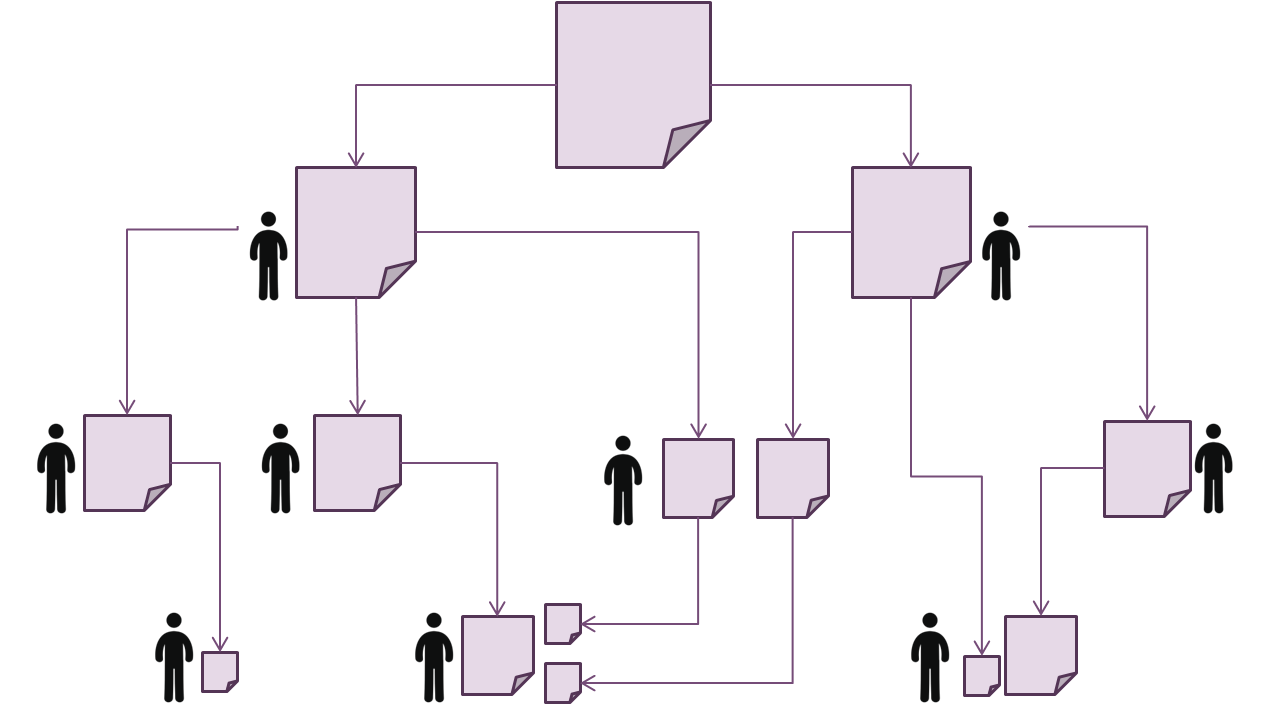
\includegraphics[width=.8\columnwidth]{src/figures/filelevel}
		\caption{A f�jlszint� hozz�f�r�s-szab�lyoz�s probl�m�ja}
		\label{fig:filelevel}
	\end{center}
\end{figure}

Erre a probl�m�ra a hozz�f�r�sek modellszint� szab�lyoz�sa ny�jt megold�st. A MONDO nemzetk�zi kutat�si projektben k�sz�lt kollabor�ci�s keretrendszer finomszemcs�s szab�lyok alapj�n v�gzi a hozz�f�r�s-vez�rl�st. Ezekben a modell elemi r�szeire, objektumokra �s azok attrib�tumaira, referenci�ira k�l�n-k�l�n lehet hozz�f�r�si jogokat meghat�rozni a k�l�nb�z� felhaszn�l�k tekintet�ben. A k�rd�ses modellelemeket gr�flek�rdez�s eredm�nyek�nt kapjuk, amely �gy is megfogalmazhat�, hogy tetsz�leges sz�m� �s tulajdons�g� elemet adjon vissza. �gy egy milli�s nagys�grend� modell eset�n nem sz�ks�ges egyes�vel minden egyes elemre le�rni a jogosults�gokat.
A finomszemcs�zetts�gb�l fakad�an a megadott szab�lyok k�z�tt el�fordulhat konfliktus, inkonzisztencia. Ezek felold�s�hoz sz�ks�ges egy olyan ki�rt�kel� komponens, ami eredm�nyk�nt az effekt�v, val�ban �rv�nyre jut� hozz�f�r�si szab�lyokat adja.
 
A szakdolgozat kidolgoz�sa sor�n kit�z�tt c�lok:
\begin{itemize}
	\item Sz�veges szintaxis defini�l�sa lek�rdez�s alap�, finomszemcs�s szab�lyok megfogalmaz�s�hoz
	\item EMF modellek felett a fenti nyelven megadott szab�lyok ki�rt�kel�s�t v�gz� algoritmus implement�l�sa, ami
	    \begin{itemize}
		    \item megvizsg�lva az explicit megadott szab�lyokat,
		    \item megtartva a modell bels� konzisztenci�j�t,
		    \item kiv�lasztja k�z�l�k azokat, amelyek �rv�nyre jutnak
	    \end{itemize}
	\item Az algoritmus m�k�d�s�nek bemutat�sa, teljes�tm�ny�nek ki�rt�kel�se egy r�szletesen kidolgozott esettanulm�nyon
\end{itemize}


%----------------------------------------------------------------------------
\chapter{Esettanulm�ny}
%----------------------------------------------------------------------------
%----------------------------------------------------------------------------
\section{Modell}
%----------------------------------------------------------------------------

Nagy, �sszetett ipari rendszerek tervez�s�ben sz�les k�rben elterjedt m�dszer a modellvez�relt szoftverfejleszt�s. Az ehhez jelenleg rendelkez�sre �ll� modellez�eszk�z�k gyakran �tk�znek sk�l�zhat�s�gi korl�tokba. A MONDO EU FP7 kutat�si projekt c�lja ezen kih�v�sok megold�sa olyan technol�gi�k, algoritmusok, eszk�z�k kifejleszt�s�vel, amelyek a mostanin�l nagyobb hat�konys�got, rugalmass�got biztos�tanak a rendszermodellez�s ter�n. A projekt nemzetk�zi ipari r�sztvev�i k�z�l egy sz�lturbinavez�rl� egys�geket �sszefog� rendszer esettanulm�ny�t vizsg�ltam. A rendszer leegyszer�s�tett strukt�r�j�t \aref{fig:metamodel} �br�n l�v� Ecore metamodell szeml�lteti.

\begin{figure}[hb]
	\begin{center}
		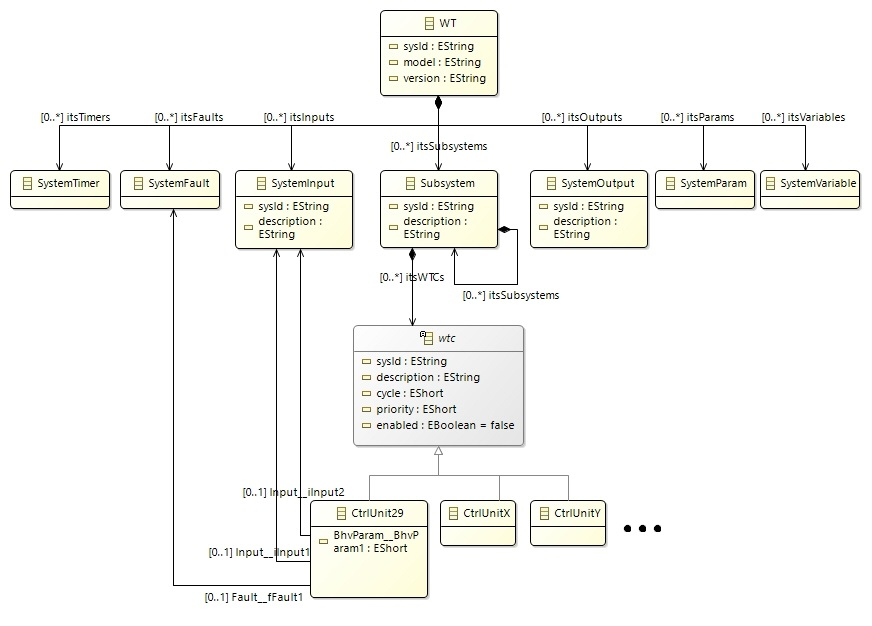
\includegraphics[width=.8\columnwidth]{src/figures/metamodel}
		\caption{Sz�lturbinavez�rl�k metamodellje}
		\label{fig:metamodel}
	\end{center}
\end{figure}

A modell gy�k�releme maga a sz�lturbina (WT - Wind Turbine), ami tov�bbi egym�sba �gyazhat� alrendszerekben (Subsystem) t�rolja a vez�rl�egys�gek (CtrlUnit - Control Unit) b�v�thet� halmaz�t az �ket azonos�t�, le�r� attrib�tumaikkal, valamint a modell t�bbi elem�re hivatkoz� referenci�ikkal. Ezek az egys�gek a megegyez� attrib�tumaikat t�rol� k�z�s �sb�l sz�rmaznak le (wtc - Wind Turbine Controller). A gy�k�relem az alrendszereken k�v�l tartalmaz m�g bemenetet, kimenetet, id�z�t�t, hibadetektort, param�tert �s v�ltoz�t (Input, Output, Timer, Fault, Param, Variable).

\begin{figure}[hb]
	\begin{center}
		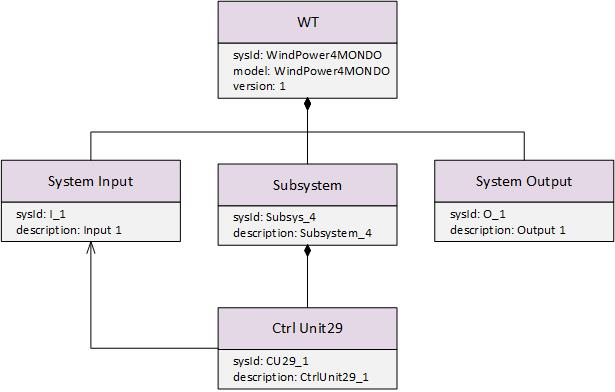
\includegraphics[width=.5\columnwidth]{src/figures/instancemodel}
		\caption{Sz�lturbinavez�rl�k p�ld�nymodellje}
		\label{fig:instancemodel}
	\end{center}
\end{figure}

A metamodell egy egyszer� p�ld�ny�t mutatja \aref{fig:instancemodel} �bra. A gy�k�relem egy vez�rl�egys�get tartalmaz egy alrendszer al� rendezve, valamint egy-egy bemenetet �s kimenetet.

%----------------------------------------------------------------------------
\section{Feladat}
%----------------------------------------------------------------------------

A modell fejleszt�se kollaborat�v m�don zajlik. Ehhez h�rom k�l�nb�z� feladatk�rrel rendelkez� felhaszn�l�t�pust defini�ltam, akiknek beoszt�suk vagy szaktud�suk alapj�n sz�ks�ges meghat�rozni, hogy a rendszer mely elemei felett rendelkezzenek olvas�si �s/vagy �r�si jogokkal. Az �rv�nyes�teni k�v�nt szab�lyok a k�vetkez�k:

\begin{itemize}
	\item A gy�k�relemet senki nem m�dos�thatja.
	\item Principal Engineer: adminisztr�tor jogokkal rendelkezik. A gy�k�relemen k�v�l mindent l�that �s m�dos�that.
	\item I/O manager: a be- �s kimenetek felel�se, ezeket olvashatja �s �rhatja, de a modell t�bbi r�sze sz�m�ra rejtett.
	\item Subsystem Manager: A Principal Engigeer-hez k�pest annyival van kevesebb joga, hogy a be- �s kimeneteket csak l�thatja, de nem m�dos�thatja.
\end{itemize} 

A feladat ezeknek a szab�lyoknak egy �ltalam defini�lt nyelven val� megfogalmaz�sa, majd a [cikk]-ben szerepl� algoritmus implement�l�sa, ami fut�s�nak eredm�nyek�pp a modell bels� konzisztenci�j�t megtartva v�logatja ki a lenti \ref{fig:instancemodelperuser} �br�n l�that� effekt�v jogosults�gokat.

\begin{figure}[t]
	\begin{center}
		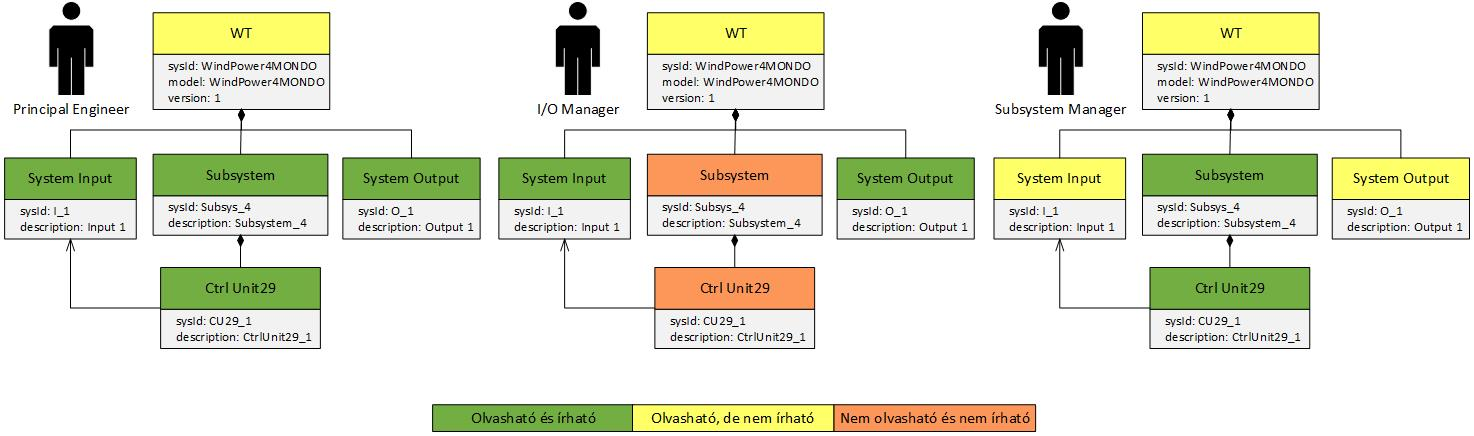
\includegraphics[width=1\columnwidth]{src/figures/instancemodelperuser}
		\caption{A felhaszn�l�k tervezett jogosults�gai}
		\label{fig:instancemodelperuser}
	\end{center}
\end{figure}
%----------------------------------------------------------------------------
\chapter{H�tt�rtechnol�gi�k, ismeretek}
%----------------------------------------------------------------------------
%----------------------------------------------------------------------------
\section{Modellez�s}
%----------------------------------------------------------------------------
%----------------------------------------------------------------------------
\subsection{Modellvez�relt szoftverfejleszt�s}
%----------------------------------------------------------------------------

Az MDE (Model-Driven Engineering) \cite{Andova2012} egy olyan szoftvertervez�si m�dszer, amelynek c�lja a rendszer magasszint� modellekkel val� le�r�sa �s az automatiz�l�s n�vel�se a fejleszt�s sor�n. A magas absztrakci�s szint a nagym�ret�, ak�r t�bb milli� k�dsort tartalmaz�, �sszetett szoftvereket �tl�that�v�, k�nnyen kezelhet�v� teszi, ugyanakkor a modellt tov�bb finom�tva a rendszer a legapr�bb r�szletekig megtervezhet�. A modellb�l t�bbek k�z�tt futtathat� forr�sk�d, tesztesetek vagy dokument�ci� is automatikusan gener�lhat�. Ez �s a magasszint� modellek tervez�s k�zbeni verifik�ci�ja cs�kkenti az implement�l�s sor�n el�fordulhat� emberi hib�k m�rt�k�t, ami k�l�n�sen el�ny�s p�ld�ul biztons�gkritikus rendszerek fejleszt�se eset�n.

A magas absztrakci�s szint� modellek el�nye, hogy k�l�nb�z� ipar�gak - informatik�hoz �s programoz�shoz nem felt�tlen�l �rt� - szak�rt�i sz�m�ra is �rthet�v� tehet�k. Azt a folyamatot, amikor a modellt egy adott szakter�let (domain) szerint tervez�nk, szakter�let-specifikus modellez�snek nevezz�k. Ilyen domain-specifikus modell az esettanulm�nyban eml�tett sz�lturbina-vez�rl�k modellje is, amit a hozz� defini�lt felhaszn�l�k ugyanolyan m�don tudnak �rtelmezni.

%----------------------------------------------------------------------------
\subsection{Eclipse Modeling Framework}
%----------------------------------------------------------------------------

Az Eclipse Modeling Framework (EMF) \cite{emf} egy modellez� �s k�dgener�l� keretrendszer domain-specifikus modellek fejleszt�s�hez. Megk�l�nb�zteti a metamodellt a t�nyleges modellt�l, el�bbi a modell strukt�r�j�t �rja le, ut�bbi a metamodell egy konkr�t p�ld�nya.

Az �gynevezett ecore f�jlban t�rolt metamodell egy UML oszt�lydiagramhoz hasonl� m�don �p�l fel. Ennek elemeit az EMF Ecore nev� (meta)metamodellje biztos�tja. Az �ltalunk elk�sz�thet� metamodell oszt�lyokat reprezent�l� EClass-okat tartalmaz, amelyek tulajdons�gait EAttribute-ok �rj�k le, a k�z�tt�k l�v� kapcsolatokat pedig EReference-ek jelzik. Ezek a referenci�k lehetnek egyszer� asszoci�ci�k vagy tartalmaz�sok is. 

Az esettanulm�ny sz�lturbina modellj�t \aref{fig:metamodel} �bra mutatja. A modell gy�k�releme maga a sz�lturbina (WT), ami tov�bbi egym�sba �gyazhat� alrendszerekben (Subsystem) t�rolja a vez�rl�egys�gek (CtrlUnit) b�v�thet� halmaz�t az �ket azonos�t�, le�r� attrib�tumokkal, valamint a modell t�bbi elem�re hivatkoz� referenci�kkal. Ezek az egys�gek a megegyez� attrib�tumaikat t�rol� k�z�s �sb�l sz�rmaznak le (wtc). A gy�k�relem az alrendszereken k�v�l tartalmaz m�g bemenetet, kimenetet, id�z�t�t, hibadetektort, param�tert �s v�ltoz�t (Input, Output, Timer, Fault, Param, Variable).

\begin{figure}[h]
	\begin{center}
		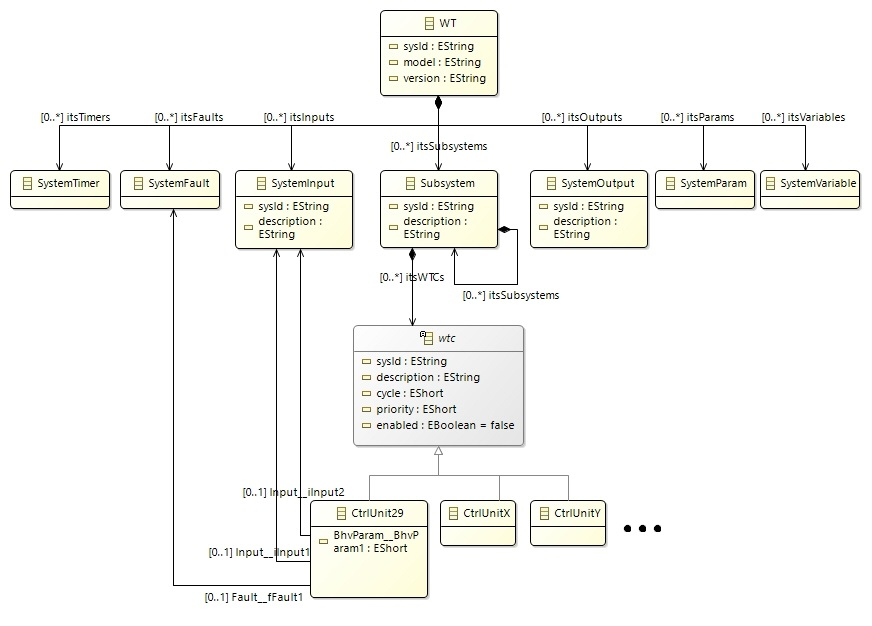
\includegraphics[width=.8\columnwidth]{src/figures/metamodel}
		\caption{Sz�lturbina-vez�rl�k metamodellje}
		\label{fig:metamodel}
	\end{center}
\end{figure}

\begin{figure}[h]
	\centering
	\begin{subfigure}[b]{0.4\textwidth}
		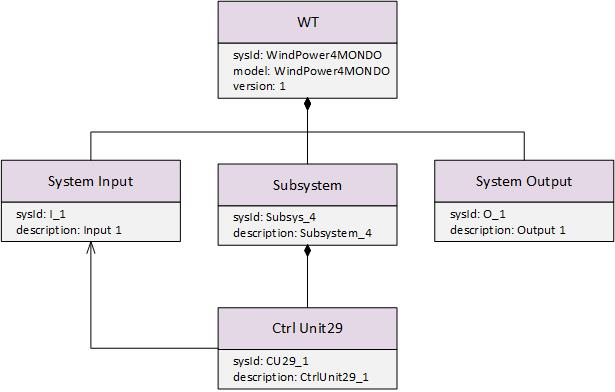
\includegraphics[width=\textwidth]{src/figures/instancemodel}
		\label{fig:instancemodel}
	\end{subfigure}
	\begin{subfigure}[b]{0.4\textwidth}
		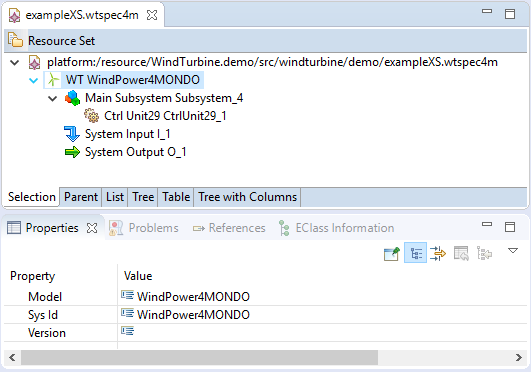
\includegraphics[width=\textwidth]{src/figures/treeeditor}
		\label{fig:treeeditor}
	\end{subfigure}
	\caption{Sz�lturbina-vez�rl�k p�ld�nymodellje}
	\label{fig:instancemodels}
\end{figure}

Az ecore metamodellb�l �jrafelhaszn�lhat� Java k�dok gener�lhat�k, t�bbek k�z�tt egy olyan fa strukt�r�j� szerkeszt� plugin, amellyel a modell k�l�nb�z� konkr�t p�ld�nyait lehet l�trehozni. A sz�lturbina-vez�rl�k metamodellj�nek egy egyszer� p�ld�ny�t mutatja \aref{fig:instancemodels} �bra, melynek jobb oldal�n l�that� az EMF alap�rtelmezett tree editorja. A gy�k�relem egy vez�rl�egys�get tartalmaz egy alrendszer al� rendezve, valamint egy-egy bemenetet �s kimenetet, amelyek k�z�l a vez�rl� az el�bbire tartalmaz referenci�t.

%----------------------------------------------------------------------------
\subsection{Modellez�si nyelvek}
%----------------------------------------------------------------------------

A modellek le�r�s�hoz szakter�let-specifikus modellez�si nyelveket haszn�lunk. Ezeknek r�szei az absztrakt szintaxis �s a konkr�t szintaxisok. El�bbi azt hat�rozza meg, hogy a nyelvnek milyen t�pus� elemei vannak �s ezek milyen kapcsolatban �llnak egym�ssal, vagyis ez maga a metamodell. Ehhez t�bb konkr�t szintaxis is megadhat� (ilyen p�ld�ul az EMF �ltal gener�lt tree editor is), amik sz�veges vagy grafikus megjelen�t�st biztos�tanak a p�ld�nymodellhez. Ezekt�l v�lik az adott szakter�let hozz��rt�i sz�m�ra olvashat�v� �s szerkeszthet�v�.

%----------------------------------------------------------------------------
\subsection{Xtext}
%----------------------------------------------------------------------------

Az Xtext keretrendszer \cite{xtext} seg�ts�g�vel sz�veges konkr�t szintaxis k�sz�thet�. Ehhez egy nyelvtant kell megadni, az ehhez tartoz� absztrakt szintaxis egy EMF modell lesz, ezt a metamodellt le tudja gener�lni a keretrendszer, �s hozz� egy egyszer� editort is ny�jt, amiben az adott nyelvtannak megfelel�en lehet fejleszteni. Ez a folyamat ford�tott ir�nyban is t�rt�nhet, m�r l�tez� ecore modellhez is gener�lhat� nyelvtan. Egy�b szolg�ltat�sai p�ld�ul a forr�sk�dsz�nez�s (syntax highlighting), hibajelz�s (validation) �s automatikus kieg�sz�t�s (content assist), ezek Java-ban val� tov�bb finom�t�s�ra is van lehet�s�g.

%----------------------------------------------------------------------------
\subsection{VIATRA Query}
%----------------------------------------------------------------------------

A VIATRA Query \cite{viatra} egy deklarat�v lek�rdez�si nyelvvel rendelkez� modelltranszform�ci�s eszk�z. A nyelv seg�ts�g�vel a lek�rdez�shez gr�fmint�kat fogalmazhatunk meg a metamodell oszt�lyaival, attrib�tumaival, referenci�ival, a rendszer pedig azokat a modellelemeket adja vissza, amelyek illeszkednek a megadott mint�ra. \Aref{code:pattern} egyszer� gr�fminta p�ld�ul a sz�lturbina-modell �sszes SystemInput t�pus� objektum�t adja vissza.

\lstinputlisting[language=viatra, caption=Egy egyszer� gr�fminta, label=code:pattern]{src/code/pattern.txt}

%----------------------------------------------------------------------------
\subsection{Bels� konzisztencia}\label{internalconsistency}
%----------------------------------------------------------------------------

Offline kollabor�ci� sor�n amikor a felhaszn�l� lek�ri a modellt a szerverr�l, akkor annak egy olyan reprezent�ci�j�t t�lti le, amiben a hozz�f�r�si szab�lyok �ltal enged�lyezett modellelemek tal�lhat�k. Ahhoz, hogy ezzel a r�szmodellel lok�lisan dolgozni tudjon (p�ld�ul v�gigiter�ljon rajta vagy soros�tsa), ennek egy teljes, �rv�nyes modellnek kell lennie. Ez �gy val�sulhat meg, ha a k�zponti modellhez hasonl�an megfelel bizonyos k�nyszereknek, amik fenntartj�k a modell bels� konzisztenci�j�t:

\begin{description}
	\item[K1\label{cons:C1}] \textbf{Objektum l�tez�se:} \\ Attrib�tumok �s referenci�k l�tez�se azt felt�telezi, hogy van m�g�tt�k egy megfelel� t�pus� objektum, ami tartalmazza �ket.
	
	\item[K2\label{cons:C2}] \textbf{Tartalmaz�si hierarchia:} \\ Ha egy objektum nem gy�k�relem, akkor tartalmazottnak kell lennie egy gy�k�relem �ltal ak�r k�zvetlen�l, ak�r k�zvetetten objektumok l�ncolat�n kereszt�l.
	
	\item[K3\label{cons:C3}] \textbf{Ellent�tes referenci�k:} \\ A k�tir�ny� referenciat�pusok p�rban p�ld�nyos�that�k.
	
	\item[K4\label{cons:C4}] \textbf{Sz�moss�gi k�nyszerek:} \\ Egy objektum adott t�pus� referenci�inak sz�ma meg kell hogy feleljen a t�pushoz defini�lt sz�moss�gnak.
\end{description}

Mivel a modell lek�r�sekor t�rt�n� modelltranszform�ci� sor�n ker�l sor a hozz�f�r�s-szab�lyoz�sra is, ez�rt a bels� konzisztencia megtart�sa azon is m�lik, hogy milyen hozz�f�r�si szab�lyok �rv�nyes�lnek a modellen.

%----------------------------------------------------------------------------
\subsection{Asset}
%----------------------------------------------------------------------------

Modellszint� hozz�f�r�si szab�lyokkal a modell logikai egys�geire hat�rozhatunk meg olvas�si �s �r�si jogosults�gokat. Ezeket a modellelemeket \cite{models16accesscontrol} alapj�n asseteknek nevezz�k, �s EMF modellek eset�n a k�vetkez�k�ppen csoportos�tjuk �ket:

\begin{itemize}
	\item \textbf{Objektum asset:} egy modellelem �s az � t�pusa, vagyis egy EObject �s egy EClass p�rosa hat�rozza meg. Az esettanulm�nyban pl. obj(I\_1, System Input).
	\item \textbf{Attrib�tum asset:} az �t tartalmaz� EObject illetve az attrib�tum nev�nek (EAttribute) �s �rt�k�nek h�rmasa alkotja, pl. attr(I\_1, description, input 1).
	\item \textbf{Referencia asset:} a kezd�- �s v�gpontj�ban l�v� modellelemek, valamint a referencia t�pusa, vagyis k�t EObject �s egy EReference h�rmasa azonos�tja mind az asszoci�ci�t �s a tartalmaz�st is, pl. ref(CU29\_1, Input\_iInput1, I\_1).
\end{itemize}

%----------------------------------------------------------------------------
\subsection{Modell obfuszk�ci�}
%----------------------------------------------------------------------------

Az obfuszk�ci� l�nyege, hogy egy k�v�l�ll�k el�l elrejteni k�v�nt inform�ci�t eltorz�tunk olyan m�don, hogy az min�l nehezebben �rtelmezhet� legyen, ugyanakkor visszafejt�s ut�n az eredeti adatot kapjuk vissza. Vagyis p�ld�ul k�t megegyez� inform�ci� obfuszk�lt �rt�ke teljesen elt�r egym�st�l, de egyedi azonos�t�jukat meg�rizve visszafejt�s ut�n is azonosak lesznek. Modellek hozz�f�r�s-kezel�s�n�l akkor haszn�lunk obfuszk�ci�t, ha egy assetnek csak a l�tez�s�re akarunk utalni an�lk�l, hogy annak tulajdons�gait l�that�v� tenn�nk. Ha objektumr�l van sz�, akkor az azonos�t� attrib�tumait is obfuszk�ljuk, a t�bbi jellemz�je pedig rejtve marad.

%----------------------------------------------------------------------------
\section{Hozz�f�r�s-szab�lyoz�s}
%----------------------------------------------------------------------------
%----------------------------------------------------------------------------
\subsection{Hozz�f�r�si szab�ly}
%----------------------------------------------------------------------------

Egy hozz�f�r�si szab�lynak \cite{models16accesscontrol} alapj�n n�gy alapvet� eleme van. Az egyik a hozz�f�r�s szintje, vagyis hogy enged�lyez�nk, tiltunk, vagy obfuszk�lunk. A m�sodik az oper�ci� t�pusa, ami olvas�s vagy �r�s lehet. Azt is meg kell hat�rozni, hogy melyik felhaszn�l�ra vagy azoknak mely csoportj�ra vonatkozik a szab�ly, valamint ki kell v�lasztanunk asseteknek azt a halmaz�t, amelyekhez szab�lyozzuk a hozz�f�r�st. \Aref{fig:accessrule} �bra azt a szab�lyt szeml�lteti, amelyben a Subsystem Manager felhaszn�l� sz�m�ra tiltjuk a System Input t�pus� modellelemek �r�s�t.

\begin{figure}[h]
	\begin{center}
		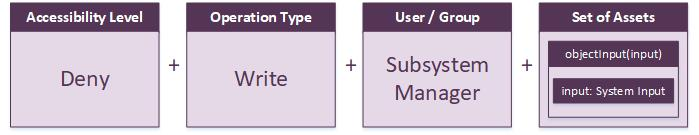
\includegraphics[width=.8\columnwidth]{src/figures/accessrule}
		\caption{Hozz�f�r�si szab�ly fel�p�t�se}
		\label{fig:accessrule}
	\end{center}
\end{figure}

Az, hogy egy szab�ly egyszerre t�bb assetre is �rtelmezhet�, gr�flek�rdez�sek seg�ts�g�vel �rhet� el. K�l�nb�z� gr�fmint�kban fogalmazzuk meg, hogy pontosan milyen tulajdons�g� elemekre van sz�ks�g�nk, a rendszer pedig visszaadja a mint�ra illeszked� tal�latokat. A szab�lyban egy ilyen gr�fmint�ra hivatkozunk, �s ak�r m�g t�bb sz�r� felt�tel megad�s�val kiv�lasztjuk a tal�latok k�z�l azokat az asseteket, amelyekre szab�lyozni akarjuk a hozz�f�r�st. A fenti szab�lyban az objectInput(input) mint�ra hivatkozunk, amely a modell �sszes System Input t�pus� objektum�t adja vissza.

Gr�flek�rdez�ssel ugyan nem kell egyes�vel defini�lni a hozz�f�r�st minden egyes assetre, viszont egy kell�en nagy modelln�l m�g assetek csoportjaira is t�l sok szab�lyt kellene megfogalmazni. Ez�rt is j� megold�s, ha a szab�lyokat egy nagyobb egys�gbe, �gynevezett policyba z�rjuk, amire megszabhatunk default jogosults�gokat. Ezeket haszn�lhatjuk, ha valamelyik modellelemre nem tal�lunk megadott hozz�f�r�st.

%----------------------------------------------------------------------------
\subsection{Szab�lyok k�z�tti konfliktusok}\label{conflicts}
%----------------------------------------------------------------------------

A hozz�f�r�si szab�lyok finomszemcs�zetts�ge miatt el�fordulhatnak k�z�tt�k az �sszer�s�g ellen sz�l� vagy a modell bels� konzisztenci�j�t megbont� konfliktusok. Ezeket \cite{commitmde16effective} szerint h�rom t�pusba soroljuk az alapj�n, hogy melyik assetre �s oper�ci�ra vonatkoznak.

\begin{itemize}
	\item \textbf{I. t�pus� konfliktus:} Ugyanarra az assetre �a ugyanarra az oper�ci�ra vonatkoz� szab�lyok ellentmond�sa, p�ld�ul egy adott assetre az egyik szab�ly enged�lyezi az olvas�st, a m�sik pedig tiltja azt.
	\item \textbf{II. t�pus� konfliktus:} Ugyanarra az assetre de k�l�nb�z� oper�ci�kra vonatkoz� szab�lyok eset�n abban az esetben fordul el�, amikor az egyik szab�ly enged�lyezi az asset m�dos�t�s�t, a m�sik viszont tiltja a l�that�s�g�t. Az �sszer�s�g �gy dikt�ln�, hogy ha egy asset �rhat�, akkor legyen olvashat� is, vagy ha nem olvashat�, akkor �rni se lehessen.
	\item \textbf{III. t�pus� konfliktus:} K�l�nb�z� assetekre �s k�l�nb�z� oper�ci�kra vonatkoz� szab�lyok a modell bels� konzisztencia k�nyszerei miatt ker�lhetnek konfliktusba egym�ssal. Ha p�ld�ul egy attrib�tum olvashat�, de az �t tartalmaz� objektum nem, az \aref{internalconsistency} r�szben eml�tett K1 konzisztencia szab�lynak mond ellent, hiszen a felhaszn�l�, akire a hozz�f�r�s vonatkozik, csak az attrib�tumot fogja l�tni a modellben, mintha nem l�tezne m�g�tte objektum. Az ilyen �s ehhez hasonl� konfliktusok felold�s�ra az olvas�si �s �r�si f�gg�s�gek bevezet�se a megold�s. A fenti esetben, ha az attrib�tumra vonatkoz� hozz�f�r�s teljes�l, akkor az �t tartalmaz� objektumra is ki kell k�nyszer�teni az olvashat�s�got.
\end{itemize}

%----------------------------------------------------------------------------
\subsection{Effekt�v jogosults�gok}
%----------------------------------------------------------------------------

A megadott hozz�f�r�sek teh�t csak nomin�lis szab�lyok, a val�ban �rv�nyre jut�, effekt�v jogosults�gok ezekt�l k�l�nb�z�ek lehetnek. A ki�rt�kel�s sor�n a modell bels� konzisztenci�j�nak megtart�sa �rdek�ben fel kell oldani a felmer�l� konfliktusokat. Ehhez a felold�shoz a szab�lyokb�l az �ltala meghat�rozott �sszes assetre el�sz�r �gynevezett judgementeket sz�rmaztatunk, amelyek \aref{fig:judgement} �br�n l�that� m�don �p�lnek fel.

A felhaszn�l� �s a default be�ll�t�s �ltal k�zvetetten megadott judgementekb�l  \aref{conflicts} r�szben eml�tett olvas�si �s �r�si f�gg�s�gek alapj�n �jabb judgementeket hat�rozunk meg. �gy kapunk egy olyan jogosults�ghalmazt, amiben a modell minden egyes assetj�re megtal�lhat�k az �rv�nyes�teni k�v�nt jogok. Ekkor jutunk el oda, hogy m�r csak azt kell vizsg�lnunk, hogy egy adott asset eset�n a k�l�nb�z� oper�ci�kra milyen enged�lyt adunk. Vagyis ezzel a m�dszerrel minden konfliktust I. t�pus�ra egyszer�s�t�nk, ami m�r k�nnyen feloldhat�.

Ehhez az I. t�pus� konfliktusfelold�shoz a judgementek az eddig eml�tett asseten, hozz�f�r�si szinten �s oper�ci�t�puson k�v�l priorit�st �s dominanci�t jelz� flaget is tartalmaznak. Az ut�bbi k�t jellemz� alapj�n d�ntj�k el, hogy melyik judgement az er�sebb, �s ez�ltal melyik fog �rv�nyre jutni a kett� k�z�l. Az els�dleges szempont a priorit�s, ezt a felhaszn�l� hozz�f�r�si szab�lyonk�nt �ll�thatja be. Ha egy priorit�si oszt�lyban vannak, akkor a dominancia d�nthet k�z�tt�k. A szab�lyokat �sszefog� policyhoz lehet enged�lyez� vagy tilt� tulajdons�got be�ll�tani, amik k�z�l az el�bbi az enged�lyez� szab�lyokat teszi domin�nss� a tilt�kkal szemben, az ut�bbi pedig ford�tva.

\begin{figure}[h]
	\begin{center}
		
\includegraphics[width=.8\columnwidth]{src/figures/judgement}
		\caption{Judgement fel�p�t�se}
		\label{fig:judgement}
	\end{center}
\end{figure}
%----------------------------------------------------------------------------
\chapter{�ttekint�s}
%----------------------------------------------------------------------------

\chapter{Megval�s�t�s}

A szakdolgozat kidolgoz�sa sor�n kit�z�tt c�lok egyike egy olyan sz�veges konkr�t szintaxis k�sz�t�se, amely lehet�v� teszi EMF modellek feletti hozz�f�r�si szab�lyok defini�l�s�t. A m�sik pedig egy olyan komponens megval�s�t�sa, ami ilyen m�don megadott szab�lyhalmazt alapul v�ve, illetve a modell bels� konzisztenci�j�nak megtart�sa �rdek�ben a
k�z�tt�k l�v� konfliktusok felold�s�val k�pes meghat�rozni az effekt�v hozz�f�r�si jogosults�gokat a modell minden egyes elem�re.

\section{Hozz�f�r�s-szab�lyoz�si nyelv}

\subsection{Nyelvtan}
Az els� feladat megold�s�t, vagyis a sz�veges konkr�t szintaxis k�sz�t�s�t egy Xtext nyelvtan defini�l�s�val kezdtem. A keretrendszer gener�lta le a hozz� tartoz� metamodellt �s sz�veges editort. \Aref{fig:impl1} �bra azt mutatja, hogy ebben a szerkeszt�ben milyen m�don lehet a specifik�lt nyelvtan alapj�n hozz�f�r�si szab�lyokat megadni. A forr�sk�dsz�nez�s be�ll�t�sa szerint a r�gz�tett kulcsszavak �s az enumer�ci�kb�l v�laszthat� �rt�kek lila sz�nnel jelennek meg, az egyedi azonos�t�sra szolg�l� nevek, sz�m�rt�kek �s a gr�flek�rdez�sek param�terei feket�vel, az id�z�jelek k�z�tt megadott stringek pedig k�kkel. Az �bra tov�bb� bekeretezve tartalmazza a felhaszn�l� �ltal megv�laszthat� param�tereket.

A rendszer felhaszn�l�it illetve a bel�l�k �ssze�ll�that� csoportokat a szab�lyok fel�r�sa el�tt kell megadni. A k�s�bbiekben mindegyik az alkalmas kulcssz� (user/group) ut�n �rt egyedi n�vvel azonos�that�. A csoport elnevez�se ut�n kapcsos z�r�jelek k�z�tt adand� meg az azt alkot� felhaszn�l�(k) list�ja.

A szab�lyokat egyetlen policy foglalja mag�ba, amelyhez a policy kulcssz� ut�n a nev�t, majd a modell �sszes elem�re vonatkoz� default jogosults�got lehet megadni. A m�sodik egy hozz�f�r�si szintb�l �s egy oper�ci�t�pusb�l �ll, ezek az AccessibilityLevel �s OperationType enumer�ci�kb�l v�laszthat�k ki. El�bbi enged�lyez�st (allow), tilt�st (deny) vagy
obfuszk�l�st (obfuscate) tesz lehet�v�, ut�bbi pedig alap�rtelmezetten vonatkozhat olvas�sra (R), �r�sra (W) vagy mindkett�re (RW). (Itt a default jogosults�gok megad�s�n�l csak a RW enged�lyezett, mert mindegyik oper�ci�t�pusra meg kell hat�rozni.) A policyt bez�r� z�r�jel ut�n a ResolutionType enumer�ci� k�tf�le eleme k�z�l kell kiv�lasztani, hogy
melyik hat�rozza meg az egyenk�nt megadott szab�lyok domin�nss�g�t. A permissive tulajdons�got v�lasztva az enged�lyez� szab�lyok lesznek er�sebbek, restrictive eset�n pedig a tilt�k.

\begin{figure}
	\centering
	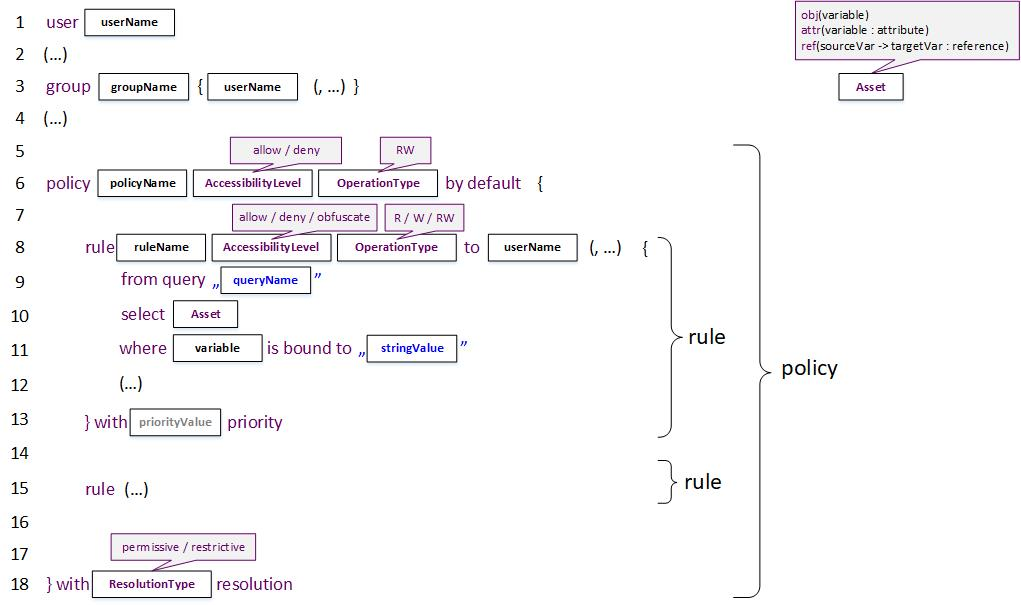
\includegraphics[width=\columnwidth]{src/figures/grammar}
	\caption{Sz�veges konkr�t szintaxis}
	\label{fig:impl1}
\end{figure}

A policyn bel�l tetsz�leges sz�m� hozz�f�r�si szab�ly le�rhat�, ezek is a rule kulcssz� ut�n �rt nev�kkel k�l�nb�ztethet�k meg. Ugyanebbe a sorba �rjuk az adni k�v�nt jogosults�g hozz�f�r�si szintj�t �s oper�ci�t�pus�t, valamint a to kulcssz� ut�n a felhaszn�l�(ka)t, aki(k)re a szab�ly vonatkozik. A szab�ly t�rzs�ben fogalmazzuk meg, hogy pontosan mely modellelemekhez adja azt a bizonyos jogosults�got. Ehhez els� l�p�sben a from query ut�n meg kell adni string form�j�ban annak a gr�fmint�nak a nev�t, amelynek az illeszked�si eredm�ny�b�l szeretn�nk kiv�lasztani a megfelel� asseteket. Ez a kiv�laszt�s a select kulcssz�val t�rt�nik, ezut�n a k�l�nb�z� t�pus� assetek a k�vetkez�k�ppen adhat�k meg:

\begin{itemize}
	\item \textbf{Objektum asset: obj(variable)} \\
	A k�v�nt objektumt�pus kiv�laszt�s�hoz a z�r�jelek k�z� kell �rni a gr�fminta param�ter v�ltoz�i k�z�l a megfelel�t.

	\item \textbf{Attrib�tum asset: attr(variable : attribute)}\\
	Az assetet a gr�flek�rdez�s eredm�nyek�nt kapott tal�lat megfelel� objektum param�tere �s egy alkalmas attrib�tuma hat�rozza meg.
		
	\item \textbf{Referencia asset: ref (sourceVar -> targetVar : reference)}\\
		A referencia k�t v�gpontja, valamint maga a referencia neve defini�lja.
\end{itemize}

A szab�ly marad�k soraiban a select-tel kiv�lasztott assetek list�ja sz�rhet� tov�bb �gy, hogy a gr�fminta megfelel� t�pus� param�ter v�ltoz�inak string �rt�k�t k�tj�k meg. Ez is er�s�ti a szab�lyok finomszemcs�zetts�g�t, hiszen �gy a legapr�bb r�szletekig tudjuk specifik�lni, hogy mely modellelemekre akarjuk meghat�rozni a hozz�f�r�si jogosults�got.

\subsection{Extra funkci�k}

A szintaxis olyan plusz funkci�kkal rendelkezik, amelyek k�nyelmesebb� teszik a fejleszt�st a szab�lyokat megad� felhaszn�l�k sz�m�ra. Az egyik ilyen az automatikus form�z�s, a megfelel� billenty�kombin�ci�t lenyomva a sz�veg \aref{code:rules} k�don l�that� m�don tagol�dik. 

Egy m�sik ilyen funkci� az �gynevezett scope provider, ami szint�n a megfelel� gyorsbillenty�re reag�lva el�hozza az adott helyre �rhat� elemek alternat�v�it. A szab�lyok fejl�c�nek v�g�n a lehets�ges felhaszn�l�kat, csoportokat, a szab�ly t�rzs�ben a from query kulcsszavak ut�n a l�tez� gr�fmint�kat aj�nlja fel. Ha megadtuk ezt a gr�fmint�t, akkor a k�vetkez� sorokban, az asset kiv�laszt�s�n�l �s a sz�r�felt�tel fogalmaz�s�n�l m�r annak a param�tereib�l lehet v�lasztani. Ha attrib�tum vagy referencia assetr�l van sz�, akkor pedig a le�rt param�ter t�pus�nak megfelel� attrib�tumokat/referenci�kat k�pes megkeresni.

A szab�lyok logikai helyess�g�nek kik�nyszer�t�s�ben pedig egy �gynevezett validator komponens seg�t. Mivel az obfuszk�ci�t csak az olvas�s m�velet�re �rtelmezz�k, m�ghozz� csak objektumok �s attrib�tumok eset�n, ez�rt a valid�ci� egyr�szt ellen�rzi, hogy szerepel-e oper�ci�t�pus a le�rt obfuscate kulcssz� ut�n, valamint hogy assetnek referenci�t adtunk-e meg. Ezen k�v�l azt is valid�lja, hogy a policy fejl�c�ben meg lett-e adva mindk�t oper�ci�t�pus (RW) a default jogosults�gok meghat�roz�s�hoz. Ezekben az esetekben a probl�m�t vil�gosan kifejez� hiba�zenettel figyelmezteti a felhaszn�l�t.

\subsection{Esettanulm�ny}
Az esettanulm�nyban felvetett hozz�f�r�s-jogosults�gi ig�nyek kiel�g�t�s�re \aref{code:rules} k�don l�that� szab�lyokat hat�roztam meg a fent bemutatott nyelven. Az �ltaluk haszn�lt gr�fmint�kat \aref{code:queries} mutatja. A h�romf�le munkak�r kifejez�s�re a PrincipalEngineer, IOManager �s SubsystemManager felhaszn�l�kat vettem fel a rendszerbe. Mivel k�z�l�k a PrincipalEnginner-nek �s a SubsystemManager-nek is t�bb objektum el�rhet�s�g�t enged�lyezz�k mint tiltjuk, ez�rt default jogosults�gnak azt adtam meg, hogy minden asset �rhat� �s olvashat�. �gy a tilt�sok kevesebb szab�lyban is �sszefoglalhat�k. Az esettanulm�nyban szerepl� k�vetelm�nyek alapj�n a k�vetkez� szab�lyokat hat�roztam meg:

\begin{itemize}
	\item restrictRoot: Az "objectRoot" lek�rdez�s a modell gy�k�relem�t adja vissza, erre
	vonjuk meg az �r�si jogot az �sszes felhaszn�l�t�l.
	\item restrictNotIO: Az "objectNotIO" a modell �sszes olyan objektum�t visszaadja, ami
	nem SystemInput vagy SystemOutput t�pus�. Ezeknek a l�that�s�g�t tiltjuk meg az
	IOManager felhaszn�l�nak.
	\item restrictIO: A Subsystem Manager sz�m�ra tiltja a SystemInput �s SystemOutput
	t�pus� objektumok m�dos�t�s�t.
	
\end{itemize}

A szab�lyokhoz priorit�st is rendeltem, a policyhoz pedig restrictive tulajdons�g tartozik, vagyis a tilt� szab�lyok sz�m�tanak er�sebbnek. Ezeknek a szab�lyokat ki�rt�kel� algoritmus m�k�d�s�ben lesz jelent�s szerep�k.

\lstinputlisting[language=rules, caption=Az esettanulm�nyhoz defini�lt hozz�f�r�si szab�lyok, label=code:rules]{src/code/policy.txt}

\lstinputlisting[language=viatra, caption=Az esettanulm�nyhoz defini�lt gr�flek�rdez�sek, label=code:queries]{src/code/query.txt}

\clearpage

\section{Szab�lyokat ki�rt�kel� komponens}

A 3.2.2 alfejezetben eml�tett k�l�nb�z� assetekre �s k�l�nb�z� oper�ci�kra vonatkoz� szab�lyok k�z�tti III. t�pus� konfliktusok felold�s�ra az olvas�si �s �r�si f�gg�s�gek bevezet�se ny�jt megold�st.

\subsection{Alapvet� f�gg�s�gek}\label{subsec:consequences}

A \cite{commitmde16effective} cikk alapj�n a megval�s�t�somban az al�bbi konfliktusok felold�s�ra vezettem be olvas�si (R) �s �r�si (W) f�gg�s�geket. Ezeket egy-egy �bra is szeml�lteti a le�r�sok ut�n, amelyekhez \aref{fig:impl2} �br�n l�v� sz�nk�dol�s tartozik. S�rga jel�li az olvashat� modellelemeket, piros a nem olvashat�kat, z�ld az �rhat�kat, k�k a nem �rhat�kat �s lila az obfuszk�ltakat.

\begin{figure}[h]
	\centering
	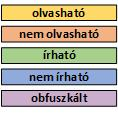
\includegraphics[width=.15\columnwidth]{src/figures/legend}
	\caption{Jelmagyar�zat}
	\label{fig:impl2}
\end{figure}

\newcommand{\conflict}[0]{$\rightarrow\leftarrow$}

\begin{description}

\item[\label{cons:f1}] \textbf{F1} Objektum olvashat� \conflict{} Attrib�tum nem olvashat� \\
A K1 konzisztencia szab�ly alapj�n az attrib�tumoknak egy-egy l�tez� objektumhoz kell tartozniuk, vagyis ha egy attrib�tum olvashat�, akkor a hozz� tartoz� objektumnak is meg kell jelennie (legal�bb obfuszk�ltan) a modelln�zetben.

\begin{figure}[h]
	\centering
	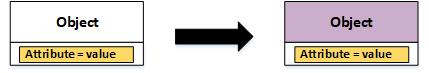
\includegraphics[width=.5\columnwidth]{src/figures/r1}
\end{figure}

\item[\label{cons:f2}] \textbf{F2} Referencia olvashat� \conflict{} Kezd�-/v�gpontbeli objektum nem olvashat�

	\begin{description}
	\item{a} Az F1 f�gg�s�ghez hasonl�an a K1 konzisztencia szab�ly kiel�g�t�s�re ha egy referencia l�that�, akkor mivel tartoznia kell k�t objektumhoz, a kezd�- �s v�gpontj�ban l�v� objektumoknak is l�that�nak kell lenni�k legal�bb obfuszk�lva.
	
	\item{b} Ezt kieg�sz�tend�, ha a forr�s vagy a c�l objektum nem olvashat�, akkor a k�z�tt�k l�v� referencia se legyen az.
	\end{description}

\begin{figure}[h]
	\begin{subfigure}[h]{\columnwidth}
		\centering
		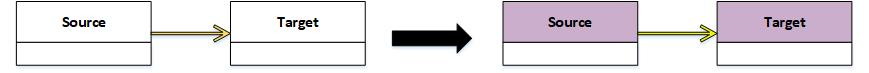
\includegraphics[width=\columnwidth]{src/figures/r2a}
		\caption{}
	\end{subfigure}
	\begin{subfigure}[h]{\columnwidth}
		\centering
		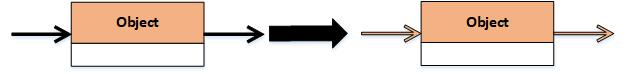
\includegraphics[width=.7\columnwidth]{src/figures/r2b}
		\caption{}
	\end{subfigure}
\end{figure}

\item[\label{cons:f3}] \textbf{F3} Objektum olvashat� \conflict{} Sz�l� objektum nem olvashat�
	\begin{description}
	\item{a} A K2 konzisztencia szab�ly �rtelm�ben ha egy objektum nem gy�k�relem, akkor egy m�sik �ltal tartalmazottnak kell lennie. Az�rt, hogy a megjelen�tett modellben l�tezzen sz�l�je, az �t tartalmaz� objektumot - ha m�s szab�ly esetleg nem engedi a l�that�s�g�t - legal�bb obfuszk�lni kell, a k�z�tt�k l�v� referenci�t pedig olvashat�v� kell tenni. T�bbsz�r�s propag�l�s ut�n ennek eredm�nyek�pp az eg�sz tartalmaz�si hierarchia megjelenik eg�szen a gy�k�relemig.
	
	\item{b} Ezt a konfliktust a m�sik oldalr�l feloldva, ha egy tartalmaz�si referencia nem l�that�, akkor a tartalmazott objektum se legyen az.
	\end{description}

\begin{figure}[h]
	\centering
	\begin{subfigure}[b]{0.45\textwidth}
		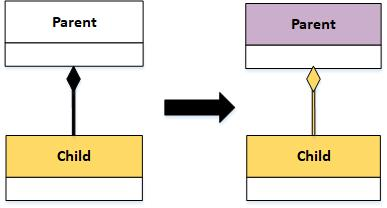
\includegraphics[width=\textwidth]{src/figures/r3a}
		\caption{}
	\end{subfigure}
	\begin{subfigure}[b]{0.45\textwidth}
		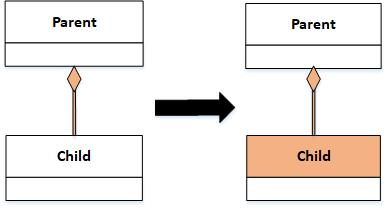
\includegraphics[width=\textwidth]{src/figures/r3b}
		\caption{}
	\end{subfigure}
\end{figure}

\item[\label{cons:f4}] \textbf{F4} Objektum olvashat� \conflict{} ID attrib�tum nem olvashat�
	\begin{description}
	\item{a} Mivel objektumok k�z�tt az egyedi azonos�t�jukkal tehet�nk k�l�nbs�get, �gy ha egy objektum l�that�, akkor az �t azonos�t� ID attrib�tum(ok)nak is olvashat�nak kell lennie.
	\item{b} Hasonl�an a m�sik ir�nyba, ha valamelyik ID attrib�tum rejtve van, akkor maga az objektum se l�tsz�dhat.
	\end{description}

\begin{figure}[h]
	\centering
	\begin{subfigure}[b]{0.6\textwidth}
		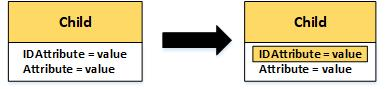
\includegraphics[width=\textwidth]{src/figures/r4a}
		\caption{}
	\end{subfigure}
    \par\bigskip
	\begin{subfigure}[b]{0.6\textwidth}
		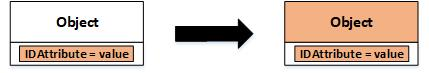
\includegraphics[width=\textwidth]{src/figures/r4b}
		\caption{}
	\end{subfigure}
\end{figure}

\item[\label{cons:f5}] \textbf{F5} Obfuszk�ci� \\
Ha egy objektum vagy attrib�tum elemre nincs meghat�rozva olvashat�s�gi enged�ly, csak az�rt szerepelnek a modellben, mert az olvas�si f�gg�s�gek kik�nyszer�tik azt, akkor obfuszk�ltan jelennek meg. Egy ilyen objektumnak az azonos�t� attrib�tumait is obfuszk�lni kell, a t�bbi attrib�tum pedig rejtve marad a modellben.

\begin{figure}
	\centering
	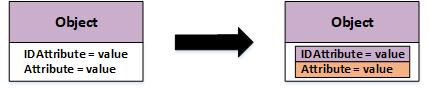
\includegraphics[width=.6\columnwidth]{src/figures/o}
\end{figure}

\item[\label{cons:f6}] \textbf{F6} Objektum �rhat� \conflict{} Tartalmaz�si referencia nem �rhat�
	\begin{description}
	\item{a} Egy objektum elt�vol�t�s�hoz nem el�g, ha � maga �rhat�, az is sz�ks�ges, hogy a r� mutat� tartalmaz�si referencia is az legyen, mert ebben az esetben azt is t�r�lni kell a modellb�l, hiszen �nmag�ban m�r nem �rtelmezhet�.
	\item{b} Ezzel �sszef�gg�sben, ha egy tartalmaz�si referencia m�dos�that�, akkor a gyerek objektumok abban az esetben t�r�lhet�k vagy �thelyezhet�k, ha �k is m�dos�that�k. Az�rt, hogy ez mindig teljes�lj�n, az algoritmus ilyen esetben is propag�lja az �rhat�s�got.
	\end{description}

\begin{figure}[h]
	\centering
	\begin{subfigure}[h]{0.45\textwidth}
		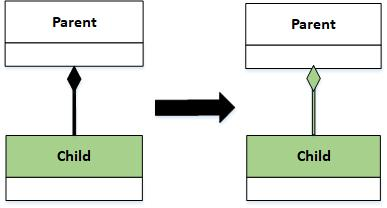
\includegraphics[width=\textwidth]{src/figures/w1a}
		\caption{}
	\end{subfigure}
	\begin{subfigure}[h]{0.45\textwidth}
		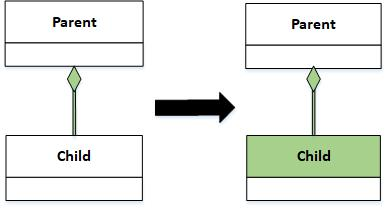
\includegraphics[width=\textwidth]{src/figures/w1b}
		\caption{}
	\end{subfigure}
\end{figure}

\item[\label{cons:f7}] \textbf{F7} ID attrib�tum �rhat� \conflict{} Tartalmaz�si referencia nem �rhat�
	\begin{description}
	\item{a} Az el�z� konfliktushelyzetet tov�bbgondolva akkor is t�rl�sre ker�l egy objektum, ha valamelyik ID attrib�tuma m�dosul. Ilyenkor elt�vol�t�s ut�n egy �j objektum ker�l a hely�re, ami m�r az �j be�ll�tott �rt�kkel rendelkezik. Teh�t ilyen attrib�tumok �rhat�s�ga eset�n erre a helyzetre felk�sz�lve az objektum tartalmaz�si referenci�j�nak is �rhat�nak kell lennie.
	\item{a} Ford�tott helyzetben ha a referencia nem m�dos�that�, akkor nem csak az objektum, hanem az azt azonos�t� attrib�tumok sem m�dos�that�k.
	\end{description}
\end{description}

\begin{figure}[h]
	\centering
	\begin{subfigure}[h]{0.45\textwidth}
		\centering
		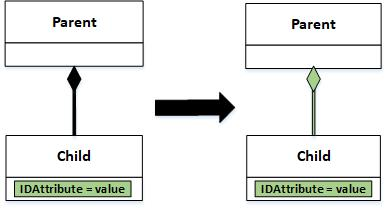
\includegraphics[width=\textwidth]{src/figures/w2a}
		\caption{}
	\end{subfigure}
	\begin{subfigure}[h]{0.45\textwidth}
		\centering
		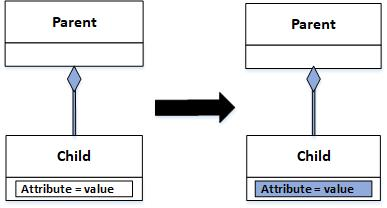
\includegraphics[width=\textwidth]{src/figures/w2b}
		\caption{}
	\end{subfigure}
\end{figure}

\clearpage

Az �r�si �s olvas�si f�gg�s�gek bevezet�s�vel nem csak a III-as, hanem a II-es t�pusba tartoz� konfliktusok is feloldhat�k. Ezek az ugyanarra az assetre �s k�l�nb�z� oper�ci�kra vonatkoz� szab�lyok k�z�tt k�t helyzetben �llnak fent, ezeket oldj�k fel az al�bbi f�gg�s�gek:

\begin{description}
	
\item[\label{cons:f8}] \textbf{F8} Asset �rhat� \conflict{} Asset nem olvashat�
	\begin{description}
	\item{a} Egy b�rmilyen asset �rhat�s�g�nak akkor van �rtelme, ha olvashat� is, hiszen hi�ba van joga a felhaszn�l�nak azt m�dos�tani, ha a sz�m�ra megjelen� modelln�zetben nincs benne az adott asset. Teh�t az �rhat�s�ggal minden asset eset�ben egy�tt kell hogy j�rjon az olvashat�s�g is.
	\item{b} Ford�tott ir�nyban, ha egy asset nem l�that�, akkor �rtelemszer�en m�dos�that� sem lehet.
	\end{description}
\item[\label{cons:f9}] \textbf{F9} Asset obfuszk�lt \conflict{} Asset �rhat� \\
Egy asset obfuszk�lts�ga eset�n k�rd�ses, hogy v�ltoztat�s ut�n mi t�rt�nik vele. Ekkor a felhaszn�l�k csak obfuszk�lt �rt�keket v�ltoztathatnak, aminek k�vetkezt�ben a vissza�ll�t�s ut�n nem felt�tlen�l a k�v�nt eredm�ny �rhet� el. Az �n megold�somban minden obfuszk�lt assetre tiltva van az �rhat�s�g.

\end{description}

\subsection{Olvas�si �s �r�si f�gg�s�gek konfigur�ci�ja}
Az implement�ci�ban egy $IConsequence$ interf�szt a $propagate()$ met�dus�val megval�s�tva a felhaszn�l� hozz�adhatja az �ltala defini�lni k�v�nt f�gg�s�geket a komponenshez. �gy a modell �rtelmess�g�t �s bels� konzisztenci�j�t t�mogat� f�gg�s�geken k�v�l ak�r m�g t�bb megk�t�ssel is konfigur�lhatja az effekt�v hozz�f�r�seket sz�m�t� algoritmust.

\clearpage

\subsection{Algoritmus m�k�d�se}
Az effekt�v hozz�f�r�si szab�lyokat kiv�laszt� f�ggv�ny a \cite{commitmde16effective} cikkben t�rgyalt megold�sb�l kiindulva az al�bbi algoritmus szerint m�k�dik.

\begin{algorithm}
	\caption{Effekt�v jogosults�gok sz�mol�sa}
	\label{alg:resolve}
	\begin{algorithmic}
		\Function{GetEffectivePermissions}{model, strongCons, weakCons, explRules, user}
		\State $permissionList\gets $ $getInitialPermissions(model, explRules, user)$
		\State $processed\gets \emptyset$
		\While{$permissionList$ is not empty}
		\State $j \gets chooseDominant(permissionList)$
		\State $processed\gets processed \cup \{j\}$
		\State $permissionList \gets permissionList \setminus \{j\}$
		\ForAll{$j' \in permissionList$}
		\If{$conflict(j, j')$} $\rhd$ I. t�pus� konfliktus eset�n igazzal t�r vissza
		\State $permissionList \gets permissionList \setminus \{j'\} $
		\EndIf
		\EndFor
		\ForAll{$strongCons$}
		\State $consequences \gets propagate(j)$
		\State $permissionList \gets permissionList \cup consequences$
		\EndFor
		\ForAll{$weakCons$}
		\State $consequences \gets propagate(j)$
		\State $permissionList \gets permissionList \cup consequences$
		\EndFor
		\EndWhile
		\EndFunction		
	\end{algorithmic}
\end{algorithm}

\begin{enumerate}
	\item \textbf{Kiindul�si judgementek list�ja:}
	\begin{enumerate}
		\item \textbf{Explicit szab�lyokb�l:} A k�v�lr�l megadott explicit hozz�f�r�si szab�lyok $permissionList$-hez val� hozz�ad�s�hoz v�gigiter�l a k�rd�ses felhaszn�l�ra vonatkoz� szab�lyokon. Minden l�p�sben l�trehozza a gr�flek�rdez�sb�l megkapott, majd a szab�lyban megfogalmazott felt�telekkel sz�k�tett assethalmaz elemeit tartalmaz� judgementeket. Ezek t�rolj�k, hogy melyik assetre, milyen oper�ci�t�pus eset�n, milyen hozz�f�r�st szeretn�nk, milyen priorit�ssal, �s hogy ez a szab�ly a policy enged�lyez� vagy tilt� tulajdons�ga alapj�n domin�ns-e vagy sem. A $permissionList$-nek a folyamat t�bbi r�sz�nek tekintet�ben is fontos tulajdons�ga, hogy az ugyanarra az assetre azonos jogosults�got ad� judgement-eket egyenl�nek veszi, �s k�z�l�k csak a nagyobb priorit�s�t tartja meg.
		\item \textbf{Default szab�lyokb�l:} A policyban meghat�rozott default jogosults�gok hozz�ad�s�hoz bej�rja a modell minden egyes objektum�t, annak attrib�tumait, referenci�it, �s az �sszes assetre, mindk�t oper�ci�t�pusra l�trehozza az adott hozz�f�r�si szint� judgementet a lehet� legkisebb priorit�ssal. �gy a default judgementekb�l �sszesen k�tszer annyi lesz mint a modellelemek sz�ma, hiszen mindegyik olvashat�s�g�r�l �s �rhat�s�g�r�l is lesz egy-egy kijelent�s.
	\end{enumerate}

    \item \textbf{Effekt�v eredm�nyek list�ja:} A $permissionList$-en k�v�l egy m�sik judgementek t�rol�s�ra szolg�l� lista is l�trej�n, a $processed$, amelybe fut�sa sor�n az algoritmus a m�r �rv�nyre jut� judgementeket helyezi.
\end{enumerate}

A judgement-list�k inicializ�l�sa ut�n megkezd�dik az effekt�v jogosults�gok sz�m�t�sa. A program egy while ciklusban hajtja v�gre azt az iter�ci�t, melynek sor�n az eredm�ny a permissionList ki�r�l�se k�zben a $processed$ list�ba ker�l, �s amelynek pontos l�p�sei a k�vetkez�k:

\begin{enumerate}[resume]
	\item \textbf{Legdomin�nsabb judgement kiv�laszt�sa:} Ez gyakorlatilag a $permissionList$ els� elem�nek kiv�tel�t jelenti, ugyanis a lista eszerint rendezett. Els�sorban a nagyobb priorit�s� elemeket veszi el�re, az azonosak k�z�l pedig az enged�lyez� vagy tilt� tulajdons�gukb�l fakad�an domin�nsak sorol�dnak a priorit�si oszt�ly elej�re. Egy elem listabeli helye hozz�ad�skor alakul ki, ekkor a program egy mapb�l olvassa ki, hogy hol van az els� ugyanilyen fontoss�g� judgement, az el� sz�rja be, majd ezek alapj�n friss�ti a mapet.
	
	\item \textbf{Kiv�lasztott judgement �thelyez�se  $permissionList$-b�l $processed$-be:} Mivel enn�l a judgementn�l nincs fontosabb a list�ban, ez�rt � mindenk�pp �rv�nyre fog jutni, �gyhogy a nomin�lis szab�lyokat tartalmaz� list�b�l �tker�l az effekt�v szab�lyok k�z�.
	
	\item \textbf{Konfliktusfelold�s:} Judgementek bevezet�s�vel k�nnyen detekt�lhat�v� v�ltak a szab�lyok k�z�tti I. t�pus� konfliktusok. A $permissionList$-en v�gigiter�lva olyan elemeket keres�nk, amelyek ugyanarra az assetre �s ugyanarra az oper�ci�t�pusra, viszont elt�r� hozz�f�r�si szintre vonatkoznak, mint a kiv�lasztott judgement. Ezeket egyszer�en kit�r�lj�k a list�b�l, hiszen m�r �gysem �rv�nyes�lhetnek.
\end{enumerate}

\Aref{subsec:consequences} fejezetr�szben felsorolt f�gg�s�geket az algoritmus "er�s" konzekvenciak�nt kezeli, vagyis ha egy judgement �rv�nyre jut, akkor a bel�le ezek alapj�n sz�rmaztatott judgementek meg�r�klik a priorit�sukat. Ennek k�sz�nhet�en mivel a k�vetkez� k�r�kben �k lesznek a legdomin�nsabbak, szint�n �rv�nyre fognak jutni. Ezeken k�v�l a program "gyenge" konzekvenci�kat is figyelembe vesz. Ezek �rtelm�ben az objektumok attrib�tumai �s referenci�i meg�r�klik az objektumhoz tartoz� hozz�f�r�si jogot, teh�t p�ld�ul ha az olvashat�, akkor az attrib�tumok, referenci�k is azok lesznek. Ezeket a judgementeket a defaultn�l nagyobb, de az er�s konzekvenci�kn�l kisebb priorit�ssal adja hozz� az algoritmus az �rv�nyes�teni k�v�nt szab�lyok halmaz�hoz, teh�t ez ut�bbi fel�l�rhatja �ket.
	
\begin{enumerate}[resume]
	\item \textbf{Er�s konzekvenci�k propag�l�sa:} A k�l�n er�s konzekvenci�kat t�rol� $strongCons$ list�n iter�lunk v�gig, �s minden $IConsequence$-t megval�s�t� oszt�ly $propagate()$ f�ggv�ny�nek eredm�ny�t, az �j judgementeket hozz�adjuk a $permissionList$-hez.
	
	\item \textbf{Gyenge konzekvenci�k propag�l�sa:} Az el�z� ponthoz hasonl�an, csak itt a $weakCons$ list�n iter�lunk v�gig.
\end{enumerate}

A k�l�nb�z� f�gg�s�gek propag�l�sa ut�n �jraindul a while cikluson bel�li folyamat, �s eg�szen addig tart, am�g a $permissionList$ ki nem �r�l. Ek�zben a $getEffectivePermissions()$ f�ggv�ny visszat�r�si �rt�ke, a $processed$ lista feltel�t�dik az effekt�v hozz�f�r�si jogokkal.

\subsection{Algoritmus �rt�kel�se}

\begin{description}
	\item[Az algoritmus termin�l.] A while ciklus addig fut, am�g a nomin�lis judgementeket tartalmaz� $permissionList$ ki nem �r�l. Ez akkor lehets�ges, ha a hozz�adhat� judgementek sz�ma v�ges. A modellelemek sz�m�nak v�gess�ge miatt a lista inicializ�l�sakor hozz�adott explicit �s default judgementek sz�ma is az lesz. A ciklus fut�sa alatt pedig a f�gg�s�gek propag�l�sa miatt b�v�l a lista, de mivel a k�dban az is szab�lyozva van, hogy olyan judgementet ne lehessen hozz�adni a $permissionList$-hez, ami m�r szerepel a $processed$-ben, ez�rt ezek sz�ma is v�ges.
	
	Ut�bbi gondolatra egy p�lda az F2 �s F3 f�gg�s�gek kapcsolata. Ha �rv�nyes�l egy tartalmaz�si referencia l�that�s�ga, akkor a gyerek objektumnak is l�that�nak kell lennie. Ha ez ut�bbi is �rv�nyes�l, akkor a propag�l�sn�l azt a judgementet adn�nk a list�hoz, hogy a r� mutat� tartalmaz�si referencia is olvashat�. Ha hozz�adn�nk, akkor ennek a kiv�laszt�s�n�l �jraindulna ez a k�r, ezt nem engedi az algoritmus.
	\item[Az algoritmus k�tszer annyi judgementet ad vissza mint az assetek sz�ma.] A k�tszeres szorz�t �gy kapjuk, hogy minden assethez egy darab olvas�si �s egy �r�si jogosults�got hat�rozunk meg, vagyis az sz�ks�ges, hogy a $processed$ list�ba minden asset mindk�t oper�ci�t�pus�hoz csak egy judgement ker�lhessen �t a $permissionList$-b�l.
	
	A judgement kiv�laszt�s�nak pillanat�ban a list�ban nem szerepel ugyanerre az oper�ci�ra �s hozz�f�r�si szintre vonatkoz� m�sik judgement, mert a list�hoz ad�skor ezt figyelembe veszi a program  �s az ilyenek k�z�l csak a magasabb priorit�s�t teszi bele. Ugyanerre az oper�ci�ra �s k�l�nb�z� hozz�f�r�si szintre vonatkoz� judgement azonban lehet benne, de a konfliktusfelold�s r�szek�nt t�rl�dnek.
	
	Felmer�lhet a k�rd�s, hogy miut�n m�r a $processed$ list�ban van az elem, egy m�sik judgement f�gg�s�geinek propag�l�sakor nem ker�lhet-e be egy ugyanolyan vagy �ppen az ellenkez�j�t kifejez� judgement a $permissionList$-be. Az ugyanolyan esetre az el�z� bizony�t�sban is szerepl� m�dszer a megold�s, vagyis arra figyel a program, hogy $processed$-ben l�v� judgement-et m�g egyszer ne adjon hozz� a list�hoz. Ellent�tes hozz�f�r�si szint� judgement pedig az �ltalam defini�lt f�gg�s�gek bizony�that� logikuss�ga miatt nem lehets�ges.
\end{description}

\clearpage

\subsection{Esettanulm�ny}
A megold�s esettanulm�nyon val� bemutat�s�hoz \aref{chap:casestudy} fejezetben meghat�rozott hozz�f�r�s-szab�lyoz�si k�vetelm�nyek alapj�n \aref{code:rules} k�don l�that� explicit �s default szab�lyok fogalmazhat�k meg. Ezek alapj�n \aref{fig:instancemodels} �br�n l�v� p�ld�nymodellen az I/O Manager felhaszn�l�ra \aref{fig:iomanagerrules}  �br�n l�that� hozz�f�r�seket szeretn�nk biztos�tani a k�l�nb�z� modellelemekhez. A gy�k�relemet csak l�thatja, de nem m�dos�thatja, a SystemInput �s SystemOutput objektumokat olvashatja �s �rhatja is, a Subsystem �s Ctrl Unit29 objektumokhoz pedig egy�ltal�n nem f�rhet hozz�. Mivel az objektumok attrib�tumaira �s referenci�ira nem adtunk meg szab�lyt, ez�rt ezekre a default be�ll�t�st �rtelmezn�nk, ami mindk�t m�veletet enged�lyezi.

\begin{figure}[h]
	\begin{center}
		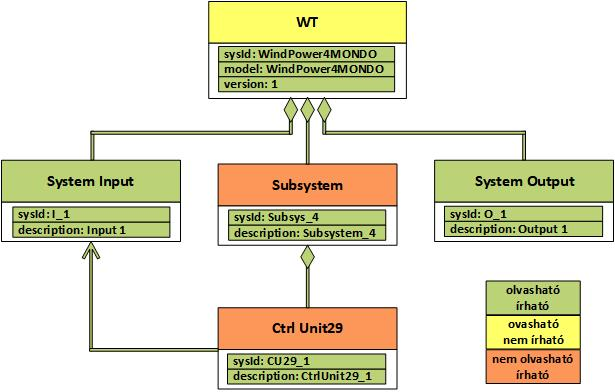
\includegraphics[width=0.6\columnwidth]{src/figures/iomanagerrules}
		\caption{Az I/O Manager sz�m�ra adni k�v�nt hozz�f�r�sek}
		\label{fig:iomanagerrules}
	\end{center}
\end{figure}

\begin{enumerate}
	\item $permissionList$ inicializ�l�sa:
	 \begin{enumerate}
	 	\item Az explicit szab�lyok k�z�l a "restrictRoot" a gy�k�relemre tiltja meg az �rhat�s�got 1-es priorit�ssal, a policy tilt� tulajdons�g�val, �gy az ebb�l sz�rmaztatott judgement:
	 	\\$j(WT, deny, W, 1, true)$
	 	\\ A m�sik r� vonatkoz� szab�ly, a "restrictNotIO" nem engedi a gy�k�relemen, bemeneteken �s kimeneteken k�v�li objektumokhoz val� hozz�f�r�st, ami ebben az esetben a k�vetkez� judgementeket eredm�nyezi:
	 	\\$j(Subsystem, deny, R, 1, true)$
	 	\\$j(Ctrl Unit29, deny, R, 1, true)$
	 	\item A default szab�lyok a modell minden assetj�re olvashat�s�got �s �rhat�s�got biztos�tanak a lehet� legkisebb, -1 priorit�ssal, �gy a k�t judgement amit mind a 21 modellelemhez rendel, �s a $permissionList$-hez az ad az algoritmus:
	 	\\$j(asset, allow, R, -1, false)$
	 	\\$j(asset, allow, W, -1, false)$
	 \end{enumerate}
 
   \item $processed$ lista inicializ�l�sa, amibe az effekt�v eredm�ny ker�l majd
\end{enumerate}

Ezek ut�n az �rv�nyes�thet� judgementek $permissionList$-b�l $processed$-be ker�l�s�nek iter�ci�nk�nti l�p�sei az al�bbiak:

\begin{enumerate}[resume]
	\item Mivel a judgementek domin�nss�ga szerint rendezett $permissionList$-be egym�s el� sz�rjuk be az ilyen szempontb�l azonos elemeket, ez�rt az els� tagja:
	\\$j(Ctrl Unit29, deny, R, 1, true)$
	
	\item Mivel ez mindenk�pp �rv�nyre jut, hozz�ad�dik a $processed$ list�hoz, feldolgoz�s ut�n pedig t�rl�dik a $permissionList$-b�l.
	
	\item Az�rt, hogy a $processed$-be ne ker�lhessen olyan judgement, ami az �pp kiv�lasztottal �s hozz�adottal konfliktusba ker�lhet, az algoritmus m�g a $permissionList$-b�l kit�rli az ugyanarra az assetre, ugyanarra az oper�ci�t�pusra, viszont m�s hozz�f�r�si szintre vonatkoz� judgement-eket. Ebben az esetben egy konfliktushelyzet ad�dik:
	\\$j(Ctrl Unit29, allow, R, -1, false)$
	\\Ez a defaultk�nt hozz�adott judgement a m�r �rv�nyre jutottal szemben enged�lyezn� a Ctrl Unit29 objektum olvashat�s�g�t, ez�rt t�rl�sre ker�l a $permissionList$-b�l.
	
	\item Az �rv�nyes�l� judgementre a k�vetkez� er�s konzekvenci�k vonatkoznak:
	\begin{itemize}
		\item F8 �rtelm�ben ha egy asset nem olvashat�, akkor �rhat� sem lehet, ez�rt a k�vetkez� judgement amit a list�hoz kell adni:
		\\$j(Ctrl Unit29, deny, W, 1, true)$
		\item F2 szerint ha egy objektum nem olvashat�, akkor a be- �s kimen� referenci�k se legyenek azok:
		\\$j(Subsystem \rightarrow Ctrl Unit29, deny, R, 1, true)$
		\\$j(Ctrl Unit29 \rightarrow SystemInput, deny, R, 1, true)$
	\end{itemize}

    \item A gyenge konzekvenci�k miatt pedig az objektum attrib�tumaira �s referenci�ira ruh�zzuk tov�bb az olvashatatlans�gi jogot a defaultn�l nagyobb, de a t�bbin�l kisebb 0 priorit�ssal. Mivel az egy sz�ba j�v� referenci�ra m�r az el�z� pontban megadtunk egy er�sebb judgementet, ez�rt arra m�r ezt felesleges lenne a list�hoz adni. Az attrib�tumokra pedig ezek vonatkoznak:
    \\$j(Ctrl Unit29.sysID, deny, R, 0, true)$
    \\$j(Ctrl Unit29.description, deny, R, 0, true)$
\end{enumerate}

A f�gg�s�gek propag�l�sa ut�n a while ciklus k�vetkez� iter�ci�ja j�n, ahol a $permissionList$-hez utolj�ra hozz�adott legdomin�nsabb judgementet v�lasztja ki az algoritmus �s teszi �t a $processed$ list�ba, ez pedig a $j(Ctrl Unit29 \rightarrow SystemInput, deny, R, 1, true)$. Konfliktusa szint�n az assethez rendelt default hozz�f�r�ssel lesz, a defini�lt f�gg�s�gek k�z�l csak az F8 vonatkozik r�, ez�rt a list�hoz azt a judgementet is hozz� kell adni, ami az asset �rhat�s�g�t tiltja.

\clearpage

A cikluson ilyen m�don addig iter�lunk v�gig, am�g a $permissionList$ �sszes elem�t fel nem dolgoztuk ak�r a $processed$ list�ba val� �thelyez�ssel, ak�r t�rl�ssel. A folyamat v�g�re az I/O Manager sz�m�ra a r� vonatkoz� effekt�v hozz�f�r�si szab�lyok alapj�n \aref{fig:iomanagerresult} �br�n l�that� konzisztens modelln�zet �rv�nyes�l.

\begin{figure}[h]
	\begin{center}
		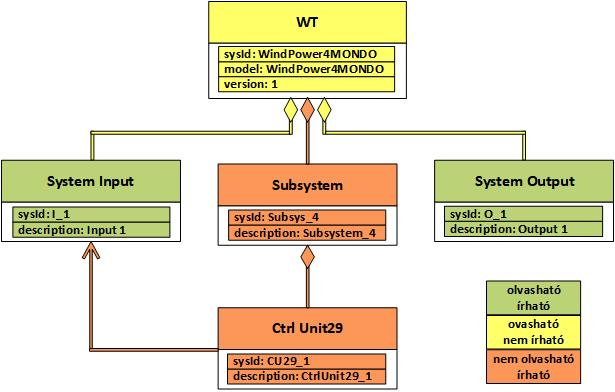
\includegraphics[width=0.6\columnwidth]{src/figures/iomanagerresult}
		\caption{Az I/O Manager sz�m�ra �rv�nyes�l� effekt�v hozz�f�r�sek}
		\label{fig:iomanagerresult}
	\end{center}
\end{figure}

Az esettanulm�nyban szerepl� m�sik k�t felhaszn�l�ra futtatva az algoritmust \aref{n} �br�n l�that� eredm�nyek sz�lettek. Bal oldalon szerepelnek a szab�lyok �ltal ig�nyelt hozz�f�r�sek, jobb oldalon pedig az algoritmus fut�si eredm�nyek�nt kapott effekt�v jogosults�gok.

\begin{figure}[h]
	\centering
	\begin{subfigure}[h]{1\textwidth}
		\centering
		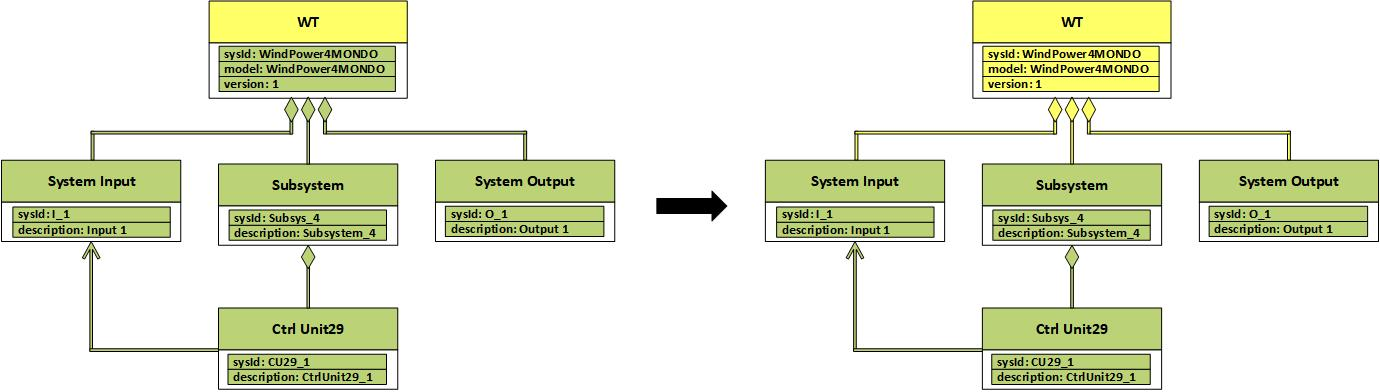
\includegraphics[width=\textwidth]{src/figures/principalengineerresult}
		\caption{Principal Engineer}
	\end{subfigure}
    \par\bigskip
	\begin{subfigure}[h]{1\textwidth}
		\centering
		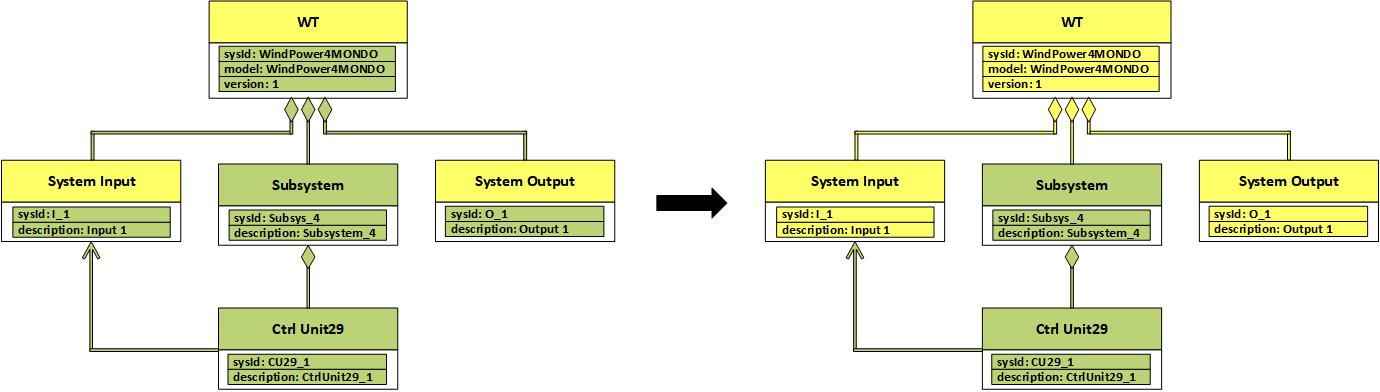
\includegraphics[width=\textwidth]{src/figures/subsystemmanagerresult}
		\caption{Subsystem Manager}
	\end{subfigure}
\end{figure}

%----------------------------------------------------------------------------
\chapter{Ki�rt�kel�s}
%----------------------------------------------------------------------------

%----------------------------------------------------------------------------
\chapter{Kapcsol�d� munk�k}
%----------------------------------------------------------------------------

%----------------------------------------------------------------------------
\chapter{�sszefoglal�s}
%----------------------------------------------------------------------------

A nagym�ret� ipari szoftverek tervez�se egy vagy ak�r t�bb c�ghez tartoz� fejleszt� csapatok egy�ttes munk�j�t ig�nyli. A modellvez�relt szoftverfejleszt�si paradigma el�nye az automatikus k�d-, teszteset-, dokument�ci�gener�l�son k�v�l, hogy az �tl�that�, magas absztrakci�s szint� modellek k�l�nf�le szakter�letekhez �rt� m�rn�k�k sz�m�ra is ugyanolyan m�don �rtelmezhet�k, ezzel �sszehangolva a k�z�s munkav�gz�st.

Ilyen komplex modellek �s ennyi k�l�nb�z� szerepk�r�, �rdekelts�g� kollabor�tor eset�n elengedhetetlen a modellek hozz�f�r�s-szab�lyoz�sa. Egyr�szt egy adott domain szakember�nek is megk�nny�ti a fejleszt�st, ha csak a sz�m�ra relev�ns r�szeit l�tja a modellnek, m�sr�szt lehetnek benne olyan bizalmas vagy kritikus elemek is, amelyekhez ide�lis esetben kiz�r�lagos joggal rendelkeznek a hozz��rt�k.

A modellszint� hozz�f�r�s-szab�lyoz�s l�nyege, hogy finomszemcs�s szab�lyokban fogalmazhatjuk meg, pontosan mely modellelemekre milyen �r�si �s olvas�si jogot szeretn�nk biztos�tani. Ezeket a szab�lyokat azonban nem tudja k�zvetlen�l felhaszn�lni az a modelltranszform�ci�, amely az adott felhaszn�l� sz�m�ra elk�sz�ti az �ltala olvashat� elemekb�l �ll� modelln�zetet, mert a szab�lyok finomhangol�si lehet�s�gei miatt ad�dhatnak k�z�tt�k olyan konfliktusok, amelyek vesz�lyeztetik a modell transzform�ci� ut�n is megtartand� bels� konzisztenci�j�t. 

A szakdolgozat c�lja egy ilyen modellszint� hozz�f�r�s-szab�lyoz�s helyes m�k�d�s�nek t�mogat�sa volt, amelyhez az al�bbi r�szfeladatokat val�s�tottam meg:

\begin{enumerate}
	\item K�sz�tettem egy hozz�f�r�si szab�lyok le�r�s�ra alkalmas sz�veges konkr�t szintaxist, amely az al�bbi jellemz�kkel rendelkezik:
	\begin{itemize}
		\item Gr�flek�rdez�ssel a szab�lyban tetsz�leges modellelemek halmaz�ra fogalmazhat� meg a jogosults�g.
		\item Finomszemcs�zett, mert a gr�flek�rdez�s ak�r egyetlen assetet is adhat eredm�nyk�nt, assethalmazra pedig tov�bbi sz�r�felt�telek is megadhat�k.
	 	\item A szab�lyok k�z�tt fontoss�gi sorrend �ll�that� fel a hozz�juk rendelt priorit�s �s a policy-hez rendelt enged�lyez� vagy tilt� tulajdons�g seg�ts�g�vel.
		\item A policy-hoz alacsony priorit�s� default hozz�f�r�si jog is defini�lhat�, amely azokra az assetekre �rv�nyes�l, amire m�s szab�ly semmit nem mond.
	\end{itemize}

    \item Megval�s�tottam a szab�lyokat EMF modellek felett ki�rt�kel� algoritmust,
    \begin{itemize}
        \item amely �rtelmezi a felhaszn�l� �ltal megadott szab�lyokat,
        \item �s a modell bels� konzisztenci�j�t a judgement-ek k�z�tti f�gg�s�gek propag�l�s�val megtartva,
    	\item a k�z�tt�k emiatt esetlegesen kialakul� konfliktusokat feloldva
    	\item a modell minden elem�re eredm�ny�l adja a hozz� tartoz�, val�ban �rv�nyes�l� olvas�si �s �r�si jogosults�gokat.
    \end{itemize}
\end{enumerate}

Az elv�gzett feladat egy tov�bbi fejleszt�si ir�nya lehet a rendszer inkrementalit�s�nak bevezet�se, hogy a szab�lyokon v�gzett kisebb v�ltoztat�s ut�n a most megval�s�tott sz�m�t�s �jrafuttat�sa n�lk�l friss�lhessen az effekt�v hozz�f�r�si jogosults�gok halmaza.

%\listoffigures\addcontentsline{toc}{chapter}{�br�k jegyz�ke}
%\listoftables\addcontentsline{toc}{chapter}{T�bl�zatok jegyz�ke}

\bibliography{bib/mybib}
\addcontentsline{toc}{chapter}{Irodalomjegyz�k}
\bibliographystyle{plain}

\label{page:last}
\end{document}
